% Phân tích chuyên sâu (1): phương pháp, dữ liệu huấn luyện, mạng. \input trong 04-thuc-nghiem.tex.
% Bảng và hình sinh bởi report/scripts/chuyen_sau/{bang,ve_hinh}.py; số trong lời phải khớp các bảng đó.
\section{Phân tích chuyên sâu: phương pháp và minh chứng}
\label{sec:cs-phuong-phap}
Các mục trước trả lời tác tử nào thắng. Phần còn lại của chương hỏi \emph{vì sao}: dữ liệu huấn luyện dạy mạng điều
gì, mỗi tác tử mắc lỗi gì ở nước nào, tìm kiếm sâu hơn sửa được loại lỗi nào, và các con số xếp hạng ổn định đến
đâu. Mọi phân tích chạy trên log và checkpoint đã có, trừ hai giải nhỏ ở Mục~\ref{sec:cs-do-nhay}. Chúng đều chạy
trên CPU của máy ở Mục~\ref{sec:cs-moi-truong}, với seed cố định.

\subsection{Môi trường và minh chứng}
\label{sec:cs-moi-truong}
Mỗi bước được chạy qua \repoFile{report/scripts/chuyen_sau/chay.py}, ghi vào
\repoFile{runs/chuyen_sau/<bước>/<thời điểm>/}: lệnh, giờ bắt đầu và kết thúc, mã thoát, commit và trạng thái cây
làm việc, phiên bản thư viện, phần cứng, bản sao mã đã chạy, toàn bộ đầu ra và mã SHA-256 của dữ liệu vào và ra.
Bảng chỉ mục các lượt ở Phụ lục~\ref{app:minh-chung}. Các bảng và hình sinh lại từ dữ liệu này, không chép tay.

\subsection{Trọng tài: bộ giải VCF}
Nhiều số đo dưới đây cần một đáp án khách quan cho câu hỏi ``thế này có thắng ép không''. Đề tài dùng bộ giải VCF ở
Mục~\ref{sec:cs-vcf-lt}: tìm theo chiều sâu, tăng dần số nước tấn công để lấy lời giải ngắn nhất, nhớ các thế đã
thất bại.
\begin{algorithm}[H]
  \caption{Tìm chuỗi VCF trong tối đa $n$ nước tấn công}
  \label{alg:cs-vcf}
  \begin{algorithmic}[1]
    \REQUIRE bên đi $M$, đối thủ $O$, số nước tấn công $n$
    \IF{$W(M,O)\neq\emptyset$}
      \RETURN thắng ngay
    \ENDIF
    \IF{$n\le1$}
      \RETURN không có
    \ENDIF
    \STATE $C\gets$ các nước tứ của $M$
    \IF{$W(O,M)\neq\emptyset$}
      \STATE $C\gets C\cap W(O,M)$ nếu $|W(O,M)|=1$, ngược lại $C\gets\emptyset$
    \ENDIF
    \FOR{$m\in C$ sao cho $W(O,M\cup\{m\})=\emptyset$}
      \IF{$|W(M\cup\{m\},O)|\ge2$}
        \RETURN thắng bằng đòn kép bắt đầu bởi $m$
      \ENDIF
      \STATE $b\gets$ ô thắng duy nhất; tìm đệ quy từ $(M\cup\{m\},\,O\cup\{b\})$ với $n-1$
      \IF{tìm được chuỗi con}
        \RETURN $m$, $b$ và chuỗi con
      \ENDIF
    \ENDFOR
    \RETURN không có
  \end{algorithmic}
\end{algorithm}
Tính chắc chắn đã chứng minh ở định lý~\ref{dl:cs-vcf}. Ngoài chứng minh, \repoFile{tests/test_vcf.py} kiểm bằng vét
cạn: trên các thế ngẫu nhiên có VCF từ hai nước trở lên, với \emph{mọi} đáp trả của bên thủ, bên công vẫn còn nước
thắng. Giới hạn độ dài là 10 nước tấn công cho bộ thế và 8 cho phân tích từng nước. Giới hạn này, cùng với việc
không xét ba hở, làm mọi số đo ``bỏ lỡ'' và ``để hở'' là cận dưới.

\section{Dữ liệu huấn luyện: hai lỗi nhãn và ảnh hưởng}
\label{sec:cs-du-lieu}
\subsection{Tổng quan tập expert\_v2}
Tập dùng để huấn luyện SL v3 (cấp 5, và gián tiếp cấp 6--8 khởi tạo từ nó) gồm các thế từ 20\,000 ván tự đấu của
Alpha-Beta độ sâu 3, sau khi loại trùng theo đối xứng. Bảng~\ref{tab:cs-mang-dulieu} và
Hình~\ref{fig:cs-mang-du-lieu} tóm tắt.
\begin{table}[H]
  \centering
  \small
  \caption{Thống kê tập dữ liệu expert\_v2 sau khi loại trùng}
  \label{tab:cs-mang-dulieu}
  \begin{tabular}{lr}
    \toprule
    Đại lượng & Giá trị \\
    \midrule
    Số thế & 297.098 \\
    Số ván & 18.822 \\
    Train / validation / test & 238.083 / 30.360 / 28.655 \\
    Thế X đi & 50,3\% \\
    Thế thuộc ván X thắng / hoà / O thắng (nhãn theo bên đi) & 46,8 / 10,0 / 43,2\% \\
    Số nước có xác suất khác 0 trong nhãn policy (TB) & 3,21 \\
    Xác suất lớn nhất trong nhãn policy (TB) & 0,706 \\
    Entropy nhãn policy (nat, TB) & 0,613 \\
    \bottomrule
  \end{tabular}
\end{table}

\begin{figure}[H]
  \centering
  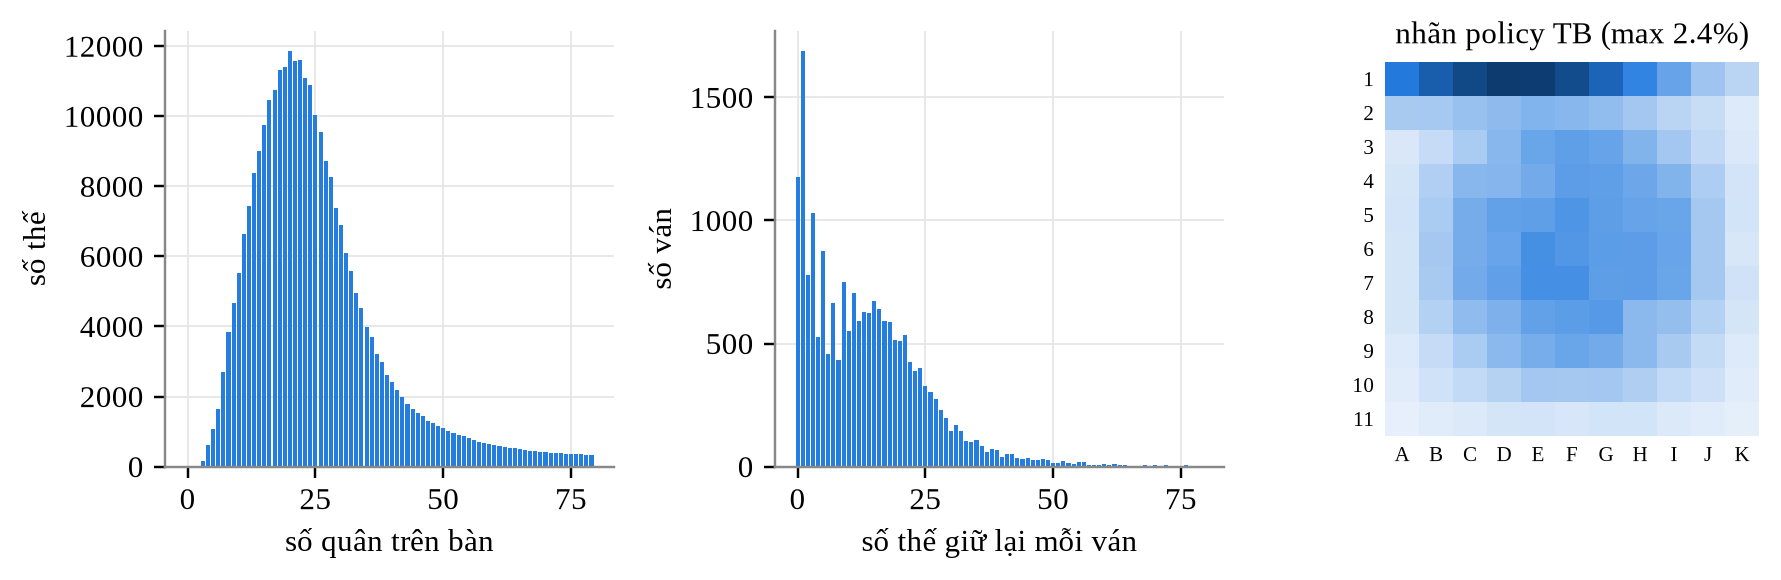
\includegraphics[width=\linewidth]{chuyen-sau/hinh/mang-du-lieu.png}
  \caption{Tập expert\_v2: phân bố số quân, số thế giữ lại của mỗi ván sau loại trùng, và nhãn policy trung bình trên
  bàn. Hàng 1 sáng bất thường dù ván diễn ra quanh tâm.}
  \label{fig:cs-mang-du-lieu}
\end{figure}
Bản đồ nhiệt bên phải là manh mối đầu tiên. Các ván bắt đầu trong vùng $5\times5$ ở giữa và nước ứng viên chỉ trong
bán kính 2 quanh quân đã có, nên xác suất cao ở hàng 1 không thể đến từ lối chơi.

\subsection{Lỗi 1: nhãn hoà điểm ở thế đã thua}
\label{sec:cs-hoa-diem}
Khi đối thủ có từ hai ô thắng và bên đi không thắng ngay được, mọi nước đều thua sau đúng một nước của đối thủ, nên
bộ tìm kiếm chấm \emph{mọi} nước cùng điểm $-(W-2)$. Hàm \texttt{scored\_moves} sắp xếp ổn định theo điểm trên danh
sách ứng viên đã theo chỉ số tăng dần (Mục~\ref{sec:cs-fail-soft} và định lý~\ref{dl:cs-topk}), nên top-5 là năm ứng
viên chỉ số nhỏ nhất; softmax của năm điểm bằng nhau là phân bố đều. Mạng được dạy rằng, khi sắp thua, nước tốt nằm
ở góc trên bên trái.

\begin{table}[H]
  \centering
  \small
  \caption{Nhãn policy hoà điểm trong hai tập dữ liệu chuyên gia}
  \label{tab:cs-dl-hoadiem}
  \begin{tabular}{lrr}
    \toprule
    Đại lượng & expert\_v1 & expert\_v2 \\
    \midrule
    Số mẫu & 27.720 & 297.098 \\
    Mẫu có nhãn hoà điểm & 12.601 & 48.043 \\
    Mẫu ở thế đã thua & 902 & 35.045 \\
    Thế đã thua có nhãn hoà & 100,0\% & 100,0\% \\
    Nước nhãn cao nhất ở hàng 1: toàn tập & 17,0\% & 14,7\% \\
    \quad trong mẫu hoà & 31,0\% & 73,8\% \\
    \quad trong mẫu không hoà & 5,4\% & 3,3\% \\
    \quad trong thế đã thua & 82,6\% & 91,9\% \\
    Nhãn hàng 1 đến từ mẫu hoà & 82,6\% & 81,3\% \\
    Ván không còn mẫu sau loại trùng & 17.242 & 1.178 \\
    Ván còn không quá 2 mẫu & 19.009 & 3.643 \\
    \bottomrule
  \end{tabular}
  \par\smallskip\parbox{.95\linewidth}{\footnotesize Hoà điểm: nhãn đặt xác suất bằng nhau lên từ hai nước trở lên. Thế đã thua: đối thủ có từ hai ô thắng, bên đi không có ô thắng.}
\end{table}

Bảng~\ref{tab:cs-dl-hoadiem} cho thấy ở tập v2, $16{,}2\%$ mẫu có nhãn đều trên nhiều nước. Mọi thế đã thua đều thuộc
loại này, và $91{,}9\%$ trong số đó có nước nhãn cao nhất nằm ở hàng 1. Tính ngược lại, $81{,}3\%$ các nhãn ``hàng 1''
của cả tập là do hoà điểm. Nguyên nhân được tái hiện trực tiếp: gọi lại cấp 3 ở độ sâu 3 trên 200 thế đã thua lấy
ngẫu nhiên từ tập, cả 200 thế mọi nước cùng một điểm và tập nước nhãn trùng đúng với tập trong dữ liệu.

\begin{table}[H]
  \centering
  \footnotesize
  \caption{Tỷ lệ nhãn hoà theo số quân trên bàn}
  \label{tab:cs-dl-theoquan}
  \begin{tabular}{lrrrrrrr}
    \toprule
    Quân & v1: mẫu & hoà & ván hoà & v2: mẫu & hoà & đã thua & ván hoà \\
    \midrule
    0--9 & 1.403 & 8,6\% & 0,6\% & 14.727 & 1,2\% & 0,0\% & 1,5\% \\
    10--19 & 4.182 & 6,3\% & 1,3\% & 90.685 & 6,2\% & 4,7\% & 1,4\% \\
    20--29 & 4.193 & 15,9\% & 1,8\% & 100.967 & 20,4\% & 17,4\% & 2,2\% \\
    30--49 & 2.143 & 10,4\% & 13,9\% & 61.245 & 21,0\% & 18,9\% & 8,9\% \\
    $\ge 50$ & 15.799 & 71,7\% & 95,5\% & 29.474 & 29,9\% & 5,4\% & 69,9\% \\
    \bottomrule
  \end{tabular}
\end{table}

Tỷ lệ nhãn hoà tăng theo số quân (Bảng~\ref{tab:cs-dl-theoquan}): càng về cuối ván càng nhiều thế đã định đoạt. Ở
tập v1 (nhiệt độ $0{,}5$), phần lớn nhãn hoà ở thế đông quân đến từ ván hoà, và 17\,242 trên 20\,000 ván không còn mẫu
nào sau loại trùng: nhiệt độ thấp khiến các ván gần như trùng nhau. Đó là lý do v2 tăng nhiệt độ lên 8.

\subsection{Lỗi 2: nhãn pha loãng ở thế thắng ngay được}
Ở thế bên đi thắng ngay được, điểm của nước thắng ngay là $W-1$, còn một nước không liên quan cũng được chấm $W-3$ vì
ván sau đó vẫn thắng ở lượt kế tiếp. Với nhiệt độ $T=8$, tỷ số trọng số softmax giữa hai mức chỉ là
$e^{-2/8}\approx0{,}78$: nước thắng chậm gần như được dạy ngang nước thắng ngay. Một thế điển hình trong dữ liệu có
hai ô thắng được chấm 999\,999, các ô chỉ số nhỏ nhất tiếp theo được chấm 999\,997 và chen vào top-5.

\begin{table}[H]
  \centering
  \small
  \caption{Nhãn ở các thế bên đi thắng ngay được (expert\_v2)}
  \label{tab:cs-dl-thangngay}
  \begin{tabular}{lr}
    \toprule
    Đại lượng & Giá trị \\
    \midrule
    Số mẫu (tỷ lệ trong tập) & 39.075 (13,2\%) \\
    Xác suất nhãn đặt trên các ô thắng (trung bình) & 47,4\% \\
    Mẫu đặt dưới 50\% lên các ô thắng & 94,7\% \\
    Nước nhãn cao nhất là ô thắng & 100,0\% \\
    Mẫu chỉ có đúng một ô thắng & 1,4\% \\
    \bottomrule
  \end{tabular}
\end{table}

Bảng~\ref{tab:cs-dl-thangngay} cho thấy $13{,}2\%$ mẫu thuộc loại này, và trung bình nhãn chỉ đặt $47{,}4\%$ xác suất
lên các ô thắng; $94{,}7\%$ mẫu đặt dưới một nửa. Nước nhãn cao nhất luôn là nước thắng, nên argmax không bị ảnh hưởng
trong dữ liệu, nhưng mạng học phân bố, không chỉ argmax. Một dấu hiệu của vòng xoáy: chỉ $1{,}4\%$ mẫu này có đúng một
ô thắng, tức expert thường bỏ qua nước thắng đủ lâu để tích thêm đe doạ, rồi chính các thế đó lại vào tập huấn luyện.

\subsection{Mạng đã học gì từ hai lỗi}
\begin{table}[H]
  \centering
  \scriptsize
  \caption{Top-1 (\%) và khối lượng policy ở hàng 1 (\%) theo nhóm mẫu test}
  \label{tab:cs-dl-mang}
  \begin{tabular}{lrrrrrrr}
    \toprule
    Mạng & Tất cả & Không hoà & Hoà & Đã thua & H1: không hoà & H1: hoà & H1: thua \\
    \midrule
    SL v3 (L5, L7) & 66,8 & 75,3 & 21,6 & 16,8 & 9,4 & 45,9 & 58,3 \\
    SL v3 không augment & 56,2 & 61,1 & 30,4 & 28,8 & 11,8 & 63,4 & 80,2 \\
    REINFORCE (L6) & 55,7 & 63,5 & 14,0 & 7,2 & 2,0 & 22,7 & 28,4 \\
    AlphaZero vòng 37 (L8) & 53,1 & 59,7 & 18,2 & 12,9 & 4,3 & 18,5 & 22,9 \\
    \bottomrule
  \end{tabular}
  \par\smallskip\parbox{.95\linewidth}{\footnotesize Cỡ nhóm: tất cả 28.655, không hoà 24.119, hoà 4.536, đã thua 3.487.}
\end{table}

\begin{table}[H]
  \centering
  \small
  \caption{Mạng trên các thế test thắng ngay được}
  \label{tab:cs-dl-mang-thang}
  \begin{tabular}{lrrr}
    \toprule
    Mạng & Mẫu & Argmax là ô thắng (\%) & Khối lượng ô thắng (\%) \\
    \midrule
    SL v3 (L5, L7) & 3.896 & 88,1 & 49,0 \\
    SL v3 không augment & 3.896 & 50,4 & 39,7 \\
    REINFORCE (L6) & 3.896 & 99,2 & 98,9 \\
    AlphaZero vòng 37 (L8) & 3.896 & 99,4 & 93,6 \\
    \bottomrule
  \end{tabular}
\end{table}

Bảng~\ref{tab:cs-dl-mang} tách số đo trên tập test theo hai nhóm. SL v3 đạt top-1 $75{,}3\%$ trên mẫu không hoà nhưng
chỉ $21{,}6\%$ trên mẫu hoà (nơi nhãn đúng chỉ là một quy ước tuỳ ý trong năm ô ngang nhau). Con số $66{,}8\%$ báo cáo
ở Bảng~\ref{tab:sl-test} và Bảng~\ref{tab:cs-mang-tong} là trung bình của hai nhóm, nên \emph{thấp hơn} khả năng dự đoán
trên các thế có đáp án thật. Cũng trên các thế đã thua, SL v3 dồn $58{,}3\%$ xác suất vào hàng 1, mạng không augment
$80{,}2\%$: mạng đã học lỗi. Hai mạng được huấn luyện tiếp bằng tự đấu dồn ít hơn hẳn (L6 $28{,}4\%$, L8
$22{,}9\%$), vì kết quả ván không thưởng cho quy ước đó.

Với thế thắng ngay (Bảng~\ref{tab:cs-dl-mang-thang}), argmax của SL v3 là một ô thắng ở $88{,}1\%$ mẫu, và nó chỉ đặt
$49\%$ xác suất lên các ô thắng, sát với $47{,}4\%$ của nhãn: mạng bắt chước nhãn khá trung thực. L6 và L8 đạt trên
$99\%$. Điều này khớp với số đo thi đấu ở Bảng~\ref{tab:cs-nuoc-loi}: L5 bỏ lỡ 60 trên 408 cơ hội thắng ngay, L6 chỉ
14/422, L8 1/603.

\paragraph{Điều chưa biết.} Các số đo trên chứng minh lỗi tồn tại và mạng học nó. Chúng \emph{không} cho biết sức
chơi sẽ tăng bao nhiêu nếu sửa: việc đó cần sinh lại dữ liệu và huấn luyện lại, ngoài phạm vi lượt này. Mọi kết quả
đấu trong báo cáo vẫn đúng với các tác tử đã đo.

\paragraph{Cách sửa đề xuất.} (i) Ở gốc \texttt{scored\_moves}, nếu có nước thắng ngay thì nhãn chỉ gồm các nước đó;
(ii) khi nhiều nước cùng điểm, chia đều xác suất cho \emph{tất cả} nước hoà thay vì $k$ nước đầu, hoặc loại thế đã
định đoạt khỏi phần học policy nhưng giữ cho value; (iii) giải hoà bằng điểm vị trí hoặc ngẫu nhiên theo seed;
(iv) bổ sung test khẳng định phân bố nhãn đối xứng trái--phải, trên--dưới khi lấy trung bình. Phép (iv) sẽ bắt được
cả hai lỗi ngay từ lần sinh dữ liệu đầu tiên.

\section{Phân tích bốn mạng policy--value}
\label{sec:cs-mang}
Bốn mạng cùng kiến trúc, khác cách huấn luyện: SL v3 có và không tăng cường đối xứng, mạng REINFORCE (L6) và mạng
AlphaZero vòng 37 (L8). Cả bốn được đo trên cùng 28\,655 thế test của expert\_v2 (chia theo ván, seed lúc huấn luyện).

\subsection{Độ khớp expert, entropy và sai số value}
\begin{table}[H]
  \centering
  \footnotesize
  \caption{Bốn mạng trên cùng tập test}
  \label{tab:cs-mang-tong}
  \begin{tabular}{lrrrrrr}
    \toprule
    Mạng & Top-1 & Top-3 & Top-5 & Entropy & MSE $v$ & Đúng dấu \\
    \midrule
    SL v3 (L5, L7) & 66,8 & 89,0 & 95,1 & 0,99 & 0,440 & 82,2 \\
    SL v3 không augment & 56,2 & 82,1 & 95,3 & 1,13 & 0,619 & 76,8 \\
    REINFORCE (L6) & 55,7 & 81,7 & 88,3 & 0,55 & 0,450 & 81,5 \\
    AlphaZero vòng 37 (L8) & 53,1 & 82,1 & 89,8 & 2,17 & 0,495 & 79,7 \\
    \bottomrule
  \end{tabular}
  \par\smallskip\parbox{.95\linewidth}{\footnotesize Top-$k$ đo mức trùng với nước tốt nhất của expert L3; L6 và L8 không được huấn luyện để bắt chước expert nên cột này không phải thước đo sức mạnh của chúng. Đúng dấu chỉ tính trên mẫu thuộc ván có thắng thua, nên cao hơn cột cùng tên ở Bảng~\ref{tab:sl-test}.}
\end{table}

Ba điểm nổi bật trong Bảng~\ref{tab:cs-mang-tong}. Thứ nhất, tăng cường đối xứng nâng top-1 hơn mười điểm và giảm MSE
từ $0{,}619$ xuống $0{,}440$; đây là phiên bản đo ngoại tuyến của A6. Thứ hai, entropy phản ánh mục tiêu huấn luyện:
REINFORCE làm policy sắc ($0{,}55$ nat), còn huấn luyện theo phân bố lượt thăm có nhiễu Dirichlet làm L8 phân tán
($2{,}17$ nat). Thứ ba, top-1 thấp của L6 và L8 \emph{không} đồng nghĩa yếu: chúng mạnh hơn L5 khi đấu, nghĩa là đã
rời khỏi lựa chọn của expert theo hướng có lợi.

\begin{figure}[H]
  \centering
  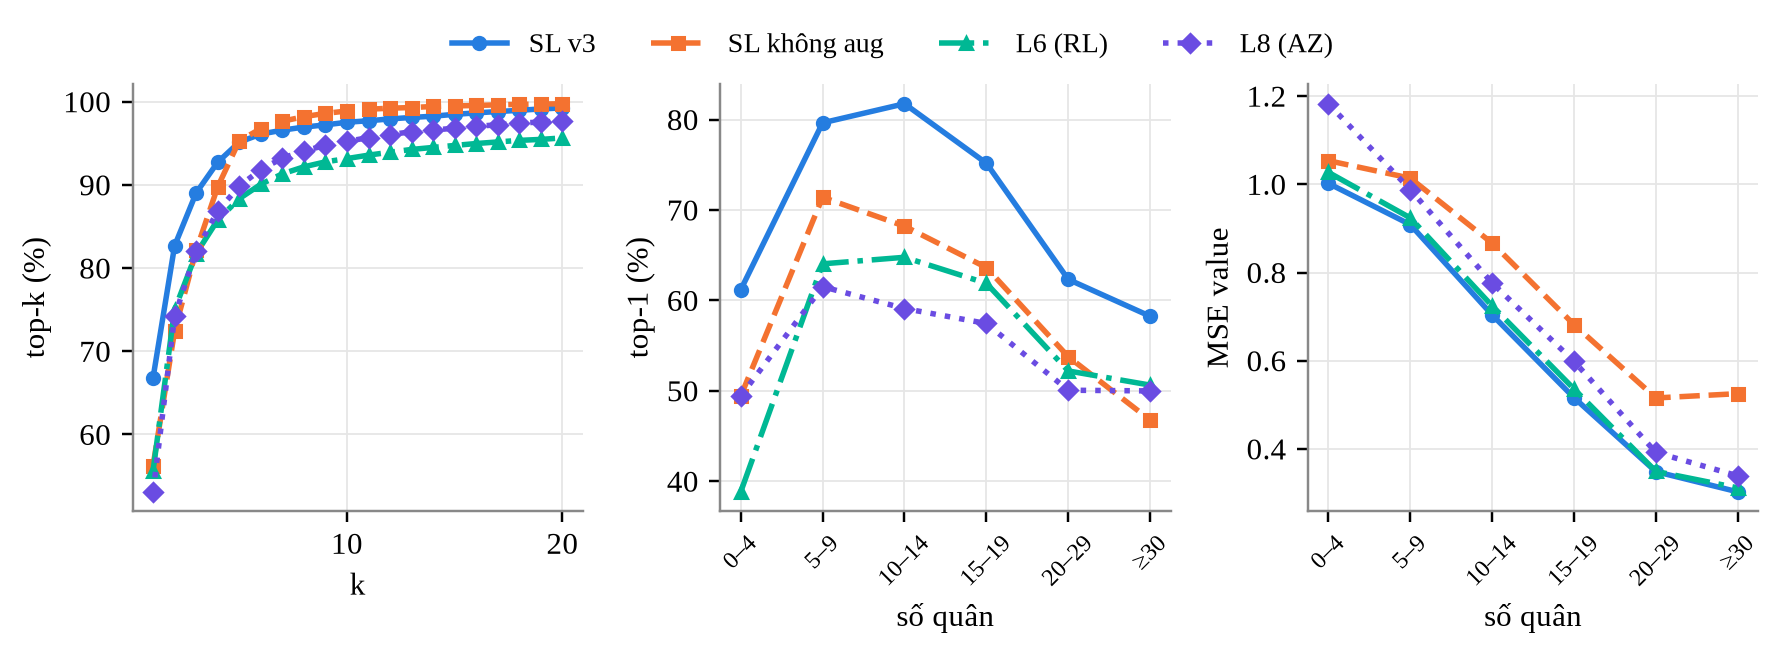
\includegraphics[width=\linewidth]{chuyen-sau/hinh/mang-giai-doan.png}
  \caption{Trái: tỷ lệ nước của expert nằm trong $k$ nước đầu của mạng. Giữa và phải: top-1 và MSE value theo số quân
  trên bàn.}
  \label{fig:cs-mang-giai-doan}
\end{figure}
\begin{table}[H]
  \centering
  \footnotesize
  \caption{Top-1 (\%) theo số quân trên bàn}
  \label{tab:cs-mang-giaidoan-top1}
  \begin{tabular}{lrrrrr}
    \toprule
    Số quân & Số thế & SL v3 & SL v3 không augment & REINFORCE & AlphaZero vòng 37 \\
    \midrule
    0--4 & 85 & 61,2 & 49,4 & 38,8 & 49,4 \\
    5--9 & 1.385 & 79,6 & 71,4 & 64,0 & 61,5 \\
    10--14 & 3.633 & 81,8 & 68,2 & 64,8 & 59,1 \\
    15--19 & 5.285 & 75,2 & 63,6 & 61,9 & 57,4 \\
    20--29 & 10.033 & 62,3 & 53,8 & 52,2 & 50,1 \\
    $\ge 30$ & 8.234 & 58,2 & 46,8 & 50,6 & 50,0 \\
    \bottomrule
  \end{tabular}
\end{table}

\begin{table}[H]
  \centering
  \footnotesize
  \caption{MSE của value theo số quân trên bàn}
  \label{tab:cs-mang-giaidoan-mse}
  \begin{tabular}{lrrrrr}
    \toprule
    Số quân & Số thế & SL v3 & SL v3 không augment & REINFORCE & AlphaZero vòng 37 \\
    \midrule
    0--4 & 85 & 1,002 & 1,054 & 1,027 & 1,183 \\
    5--9 & 1.385 & 0,909 & 1,014 & 0,924 & 0,988 \\
    10--14 & 3.633 & 0,704 & 0,866 & 0,724 & 0,776 \\
    15--19 & 5.285 & 0,516 & 0,682 & 0,536 & 0,599 \\
    20--29 & 10.033 & 0,348 & 0,516 & 0,349 & 0,392 \\
    $\ge 30$ & 8.234 & 0,303 & 0,525 & 0,312 & 0,339 \\
    \bottomrule
  \end{tabular}
\end{table}

Top-1 đạt đỉnh ở 10--14 quân ($81{,}8\%$ với SL v3) rồi giảm: cuối ván có nhiều thế hoà điểm (Lỗi 1) và nhiều nước
tương đương. MSE value giảm đều theo số quân, từ khoảng 1 ở đầu ván, tức không hơn đoán 0, xuống $0{,}30$ khi bàn
đông. Điều này đúng như định lý~\ref{dl:cs-mse}: đầu ván, phương sai không giảm được của kết quả chiếm gần hết sai số.

\subsection{Calibration của value}
\begin{figure}[H]
  \centering
  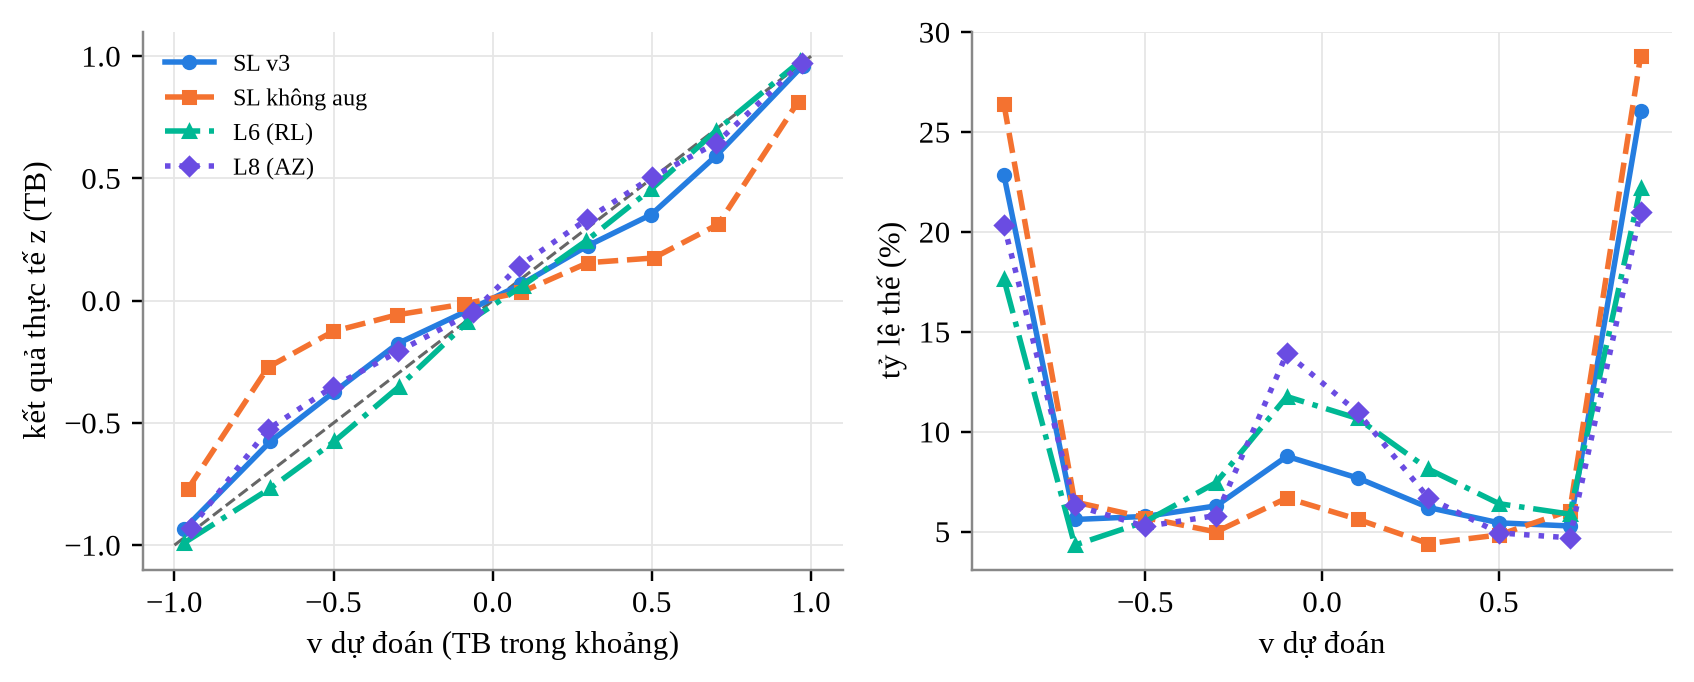
\includegraphics[width=\linewidth]{chuyen-sau/hinh/mang-calib.png}
  \caption{Trái: kết quả trung bình thực tế theo giá trị dự đoán (đường chéo là calibrated hoàn hảo). Phải: phân bố giá
  trị dự đoán.}
  \label{fig:cs-mang-calib}
\end{figure}
\begin{table}[H]
  \centering
  \footnotesize
  \caption{Kết quả trung bình thực tế $\bar z$ (số thế) theo khoảng giá trị mạng dự đoán}
  \label{tab:cs-mang-calib}
  \begin{tabular}{lrrrr}
    \toprule
    Khoảng $v$ & SL v3 & SL v3 không augment & REINFORCE & AlphaZero vòng 37 \\
    \midrule
    {}[-1,0; -0,8) & -0,94 (6.547) & -0,77 (7.564) & -0,99 (5.055) & -0,93 (5.831) \\
    {}[-0,8; -0,6) & -0,58 (1.608) & -0,27 (1.860) & -0,77 (1.240) & -0,53 (1.812) \\
    {}[-0,6; -0,4) & -0,37 (1.652) & -0,13 (1.634) & -0,58 (1.578) & -0,35 (1.508) \\
    {}[-0,4; -0,2) & -0,18 (1.803) & -0,06 (1.430) & -0,35 (2.137) & -0,21 (1.665) \\
    {}[-0,2; 0,0) & -0,04 (2.514) & -0,01 (1.916) & -0,09 (3.371) & -0,05 (3.989) \\
    {}[0,0; 0,2) & 0,07 (2.204) & 0,03 (1.611) & 0,06 (3.057) & 0,14 (3.146) \\
    {}[0,2; 0,4) & 0,22 (1.780) & 0,16 (1.263) & 0,24 (2.331) & 0,33 (1.919) \\
    {}[0,4; 0,6) & 0,35 (1.560) & 0,17 (1.387) & 0,46 (1.835) & 0,50 (1.416) \\
    {}[0,6; 0,8) & 0,59 (1.515) & 0,31 (1.737) & 0,69 (1.685) & 0,64 (1.345) \\
    {}[0,8; 1,0) & 0,96 (7.472) & 0,81 (8.253) & 0,98 (6.366) & 0,97 (6.024) \\
    \bottomrule
  \end{tabular}
\end{table}

Phân bố dự đoán của cả bốn mạng dồn về hai đầu, vì nhiều thế cuối ván đã định đoạt. Mạng không augment lệch rõ nhất:
trong khoảng dự đoán $[0{,}6;0{,}8)$, kết quả thực trung bình chỉ $0{,}31$, tức quá tự tin. SL v3 bám đường chéo tốt hơn,
vẫn hơi quá tự tin ở khoảng $[0{,}4;0{,}6)$ (thực tế $0{,}35$). L6 và L8 gần đường chéo hơn ở các khoảng dương giữa. Lưu ý
nhãn ở đây là kết quả của \emph{expert} đánh tiếp; một mạng mạnh hơn expert có thể ``sai'' theo nhãn này mà đúng với lối
chơi của chính nó.

\subsection{Đối xứng D4: tăng cường dữ liệu làm được gì}
\begin{table}[H]
  \centering
  \footnotesize
  \caption{Độ nhất quán dưới 8 phép đối xứng D4 (4.000 thế test)}
  \label{tab:cs-mang-doixung}
  \begin{tabular}{lrrrrrr}
    \toprule
    Mạng & TV & Trùng top-1 & $\sigma_v$ & Biên độ $v$ & Top-1 đơn & Top-1 TB 8 \\
    \midrule
    SL v3 (L5, L7) & 0,141 & 71,8 & 0,109 & 0,339 & 67,8 & 69,9 \\
    SL v3 không augment & 0,406 & 52,1 & 0,308 & 0,899 & 56,1 & 60,1 \\
    REINFORCE (L6) & 0,277 & 68,6 & 0,087 & 0,270 & 55,6 & 56,1 \\
    AlphaZero vòng 37 (L8) & 0,170 & 71,8 & 0,087 & 0,269 & 52,8 & 54,5 \\
    \bottomrule
  \end{tabular}
  \par\smallskip\parbox{.95\linewidth}{\footnotesize TV: khoảng cách biến phân toàn phần giữa policy gốc và policy của thế đã biến đổi (đưa về hệ toạ độ gốc). Mạng đẳng biến hoàn hảo có TV bằng 0 và trùng top-1 100\%.}
\end{table}

Bảng~\ref{tab:cs-mang-doixung} đo điều mà A6 chỉ thấy gián tiếp. Không augment, cùng một thế quay hay lật cho nước
top-1 khác nhau gần một nửa số lần (trùng $52{,}1\%$) và value dao động trung bình $0{,}90$ giữa hướng cao nhất và thấp
nhất. Augment giảm khoảng cách biến phân từ $0{,}406$ xuống $0{,}141$, nhưng chưa về 0: đẳng biến học được chỉ là xấp
xỉ. Một quan sát ngoài dự kiến: L6 xuất phát từ SL v3 ($0{,}141$) nhưng có TV $0{,}277$. Vòng REINFORCE không dùng phép
đối xứng nào, và đã làm mất một phần tính đối xứng học được trước đó. L8, có augment trong replay, giữ ở $0{,}170$.

Lấy trung bình tám hướng (định lý~\ref{dl:cs-d4}) tăng top-1 của mọi mạng, nhiều nhất ở mạng ít đối xứng (không augment
$56{,}1\to60{,}1\%$), ít ở mạng đã đối xứng. Cái giá là tám lần suy luận; đề tài không dùng nó khi thi đấu và chưa đo
tác động lên sức chơi.

\subsection{Mạng trên bộ thế chiến thuật}
Bộ thế mô tả ở Mục~\ref{sec:cs-chien-thuat}. Ở đây chỉ dùng đầu ra thô của mạng, không tìm kiếm.
\begin{table}[H]
  \centering
  \small
  \caption{Khối lượng policy (\%) đặt lên các đáp án của bộ chiến thuật}
  \label{tab:cs-mang-ct-khoiluong}
  \begin{tabular}{lrrrrr}
    \toprule
    Mạng & C1 & C2 & C3 & C4 & C5 \\
    \midrule
    SL v3 (L5, L7) & 54,7 & 98,1 & 94,1 & 82,8 & 90,2 \\
    SL v3 không augment & 42,3 & 94,7 & 81,7 & 74,4 & 83,1 \\
    REINFORCE (L6) & 89,1 & 99,1 & 96,5 & 82,1 & 92,3 \\
    AlphaZero vòng 37 (L8) & 84,8 & 76,5 & 90,2 & 62,1 & 66,6 \\
    \bottomrule
  \end{tabular}
\end{table}

\begin{table}[H]
  \centering
  \small
  \caption{Nước policy cao nhất đúng đáp án (\%) trên bộ chiến thuật}
  \label{tab:cs-mang-ct-top1}
  \begin{tabular}{lrrrrr}
    \toprule
    Mạng & C1 & C2 & C3 & C4 & C5 \\
    \midrule
    SL v3 (L5, L7) & 80,0 & 99,0 & 99,0 & 90,0 & 93,0 \\
    SL v3 không augment & 55,0 & 97,0 & 89,0 & 85,0 & 89,0 \\
    REINFORCE (L6) & 90,0 & 99,0 & 97,0 & 84,0 & 93,0 \\
    AlphaZero vòng 37 (L8) & 97,0 & 99,0 & 99,0 & 80,0 & 93,0 \\
    \bottomrule
  \end{tabular}
\end{table}

\begin{table}[H]
  \centering
  \small
  \caption{Giá trị $v$ trung bình của mạng trên từng loại thế}
  \label{tab:cs-mang-ct-value}
  \begin{tabular}{lrrrrr}
    \toprule
    Mạng & C1 & C2 & C3 & C4 & C5 \\
    \midrule
    SL v3 (L5, L7) & 0,74 & -0,12 & 0,90 & 0,71 & -0,25 \\
    SL v3 không augment & 0,60 & -0,29 & 0,81 & 0,53 & -0,21 \\
    REINFORCE (L6) & 0,86 & -0,03 & 0,85 & 0,59 & -0,17 \\
    AlphaZero vòng 37 (L8) & 0,85 & -0,20 & 0,90 & 0,46 & -0,31 \\
    \bottomrule
  \end{tabular}
\end{table}

Trên các thế thắng ngay (C1), SL v3 chỉ chọn đúng $80\%$ dù đáp án là nước hiển nhiên nhất của luật chơi: dấu vết trực
tiếp của Lỗi 2. Chặn (C2) gần như hoàn hảo ở cả bốn mạng; tạo đòn kép (C3) cũng vậy, trừ mạng không augment ($89\%$). Value nhận đúng dấu ở C1, C3, C4 (bên đi
đang thắng ép), nhưng trung bình chỉ $0{,}46$--$0{,}71$ ở C4, các chuỗi dài. Ở C2, giá trị đúng không xác định (chặn
xong có thể vẫn cân bằng), và mạng trả giá trị gần 0 hơi âm.

\begin{figure}[H]
  \centering
  \begin{subfigure}[t]{.48\linewidth}
    \centering
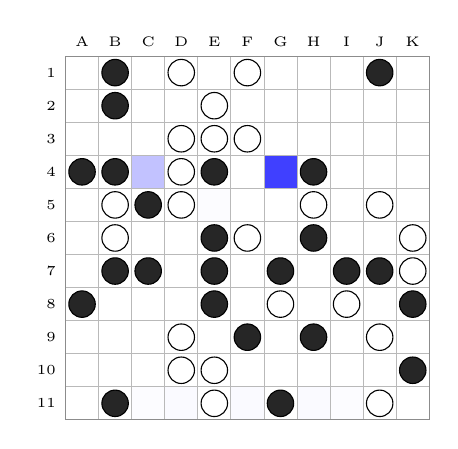
\begin{tikzpicture}[x=0.42cm, y=0.42cm]
\fill[blue!24] (2,-3) rectangle (3,-4);
\fill[blue!75] (6,-3) rectangle (7,-4);
\fill[blue!1] (4,-4) rectangle (5,-5);
\fill[blue!1] (2,-10) rectangle (3,-11);
\fill[blue!2] (3,-10) rectangle (4,-11);
\fill[blue!2] (5,-10) rectangle (6,-11);
\fill[blue!2] (7,-10) rectangle (8,-11);
\fill[blue!1] (8,-10) rectangle (9,-11);
\draw[gray!55, line width=.3pt, step=1] (0,0) grid (11,-11);
\draw[gray!90] (0,0) rectangle (11,-11);
\node[font=\tiny, anchor=south] at (0.5,0) {A};
\node[font=\tiny, anchor=south] at (1.5,0) {B};
\node[font=\tiny, anchor=south] at (2.5,0) {C};
\node[font=\tiny, anchor=south] at (3.5,0) {D};
\node[font=\tiny, anchor=south] at (4.5,0) {E};
\node[font=\tiny, anchor=south] at (5.5,0) {F};
\node[font=\tiny, anchor=south] at (6.5,0) {G};
\node[font=\tiny, anchor=south] at (7.5,0) {H};
\node[font=\tiny, anchor=south] at (8.5,0) {I};
\node[font=\tiny, anchor=south] at (9.5,0) {J};
\node[font=\tiny, anchor=south] at (10.5,0) {K};
\node[font=\tiny, anchor=east] at (0,-0.5) {1};
\node[font=\tiny, anchor=east] at (0,-1.5) {2};
\node[font=\tiny, anchor=east] at (0,-2.5) {3};
\node[font=\tiny, anchor=east] at (0,-3.5) {4};
\node[font=\tiny, anchor=east] at (0,-4.5) {5};
\node[font=\tiny, anchor=east] at (0,-5.5) {6};
\node[font=\tiny, anchor=east] at (0,-6.5) {7};
\node[font=\tiny, anchor=east] at (0,-7.5) {8};
\node[font=\tiny, anchor=east] at (0,-8.5) {9};
\node[font=\tiny, anchor=east] at (0,-9.5) {10};
\node[font=\tiny, anchor=east] at (0,-10.5) {11};
\draw[fill=black!85, line width=.4pt] (1.5,-0.5) circle (.40);
\draw[fill=white, line width=.4pt] (3.5,-0.5) circle (.40);
\draw[fill=white, line width=.4pt] (5.5,-0.5) circle (.40);
\draw[fill=black!85, line width=.4pt] (9.5,-0.5) circle (.40);
\draw[fill=black!85, line width=.4pt] (1.5,-1.5) circle (.40);
\draw[fill=white, line width=.4pt] (4.5,-1.5) circle (.40);
\draw[fill=white, line width=.4pt] (3.5,-2.5) circle (.40);
\draw[fill=white, line width=.4pt] (4.5,-2.5) circle (.40);
\draw[fill=white, line width=.4pt] (5.5,-2.5) circle (.40);
\draw[fill=black!85, line width=.4pt] (0.5,-3.5) circle (.40);
\draw[fill=black!85, line width=.4pt] (1.5,-3.5) circle (.40);
\draw[fill=white, line width=.4pt] (3.5,-3.5) circle (.40);
\draw[fill=black!85, line width=.4pt] (4.5,-3.5) circle (.40);
\draw[fill=black!85, line width=.4pt] (7.5,-3.5) circle (.40);
\draw[fill=white, line width=.4pt] (1.5,-4.5) circle (.40);
\draw[fill=black!85, line width=.4pt] (2.5,-4.5) circle (.40);
\draw[fill=white, line width=.4pt] (3.5,-4.5) circle (.40);
\draw[fill=white, line width=.4pt] (7.5,-4.5) circle (.40);
\draw[fill=white, line width=.4pt] (9.5,-4.5) circle (.40);
\draw[fill=white, line width=.4pt] (1.5,-5.5) circle (.40);
\draw[fill=black!85, line width=.4pt] (4.5,-5.5) circle (.40);
\draw[fill=white, line width=.4pt] (5.5,-5.5) circle (.40);
\draw[fill=black!85, line width=.4pt] (7.5,-5.5) circle (.40);
\draw[fill=white, line width=.4pt] (10.5,-5.5) circle (.40);
\draw[fill=black!85, line width=.4pt] (1.5,-6.5) circle (.40);
\draw[fill=black!85, line width=.4pt] (2.5,-6.5) circle (.40);
\draw[fill=black!85, line width=.4pt] (4.5,-6.5) circle (.40);
\draw[fill=black!85, line width=.4pt] (6.5,-6.5) circle (.40);
\draw[fill=black!85, line width=.4pt] (8.5,-6.5) circle (.40);
\draw[fill=black!85, line width=.4pt] (9.5,-6.5) circle (.40);
\draw[fill=white, line width=.4pt] (10.5,-6.5) circle (.40);
\draw[fill=black!85, line width=.4pt] (0.5,-7.5) circle (.40);
\draw[fill=black!85, line width=.4pt] (4.5,-7.5) circle (.40);
\draw[fill=white, line width=.4pt] (6.5,-7.5) circle (.40);
\draw[fill=white, line width=.4pt] (8.5,-7.5) circle (.40);
\draw[fill=black!85, line width=.4pt] (10.5,-7.5) circle (.40);
\draw[fill=white, line width=.4pt] (3.5,-8.5) circle (.40);
\draw[fill=black!85, line width=.4pt] (5.5,-8.5) circle (.40);
\draw[fill=black!85, line width=.4pt] (7.5,-8.5) circle (.40);
\draw[fill=white, line width=.4pt] (9.5,-8.5) circle (.40);
\draw[fill=white, line width=.4pt] (3.5,-9.5) circle (.40);
\draw[fill=white, line width=.4pt] (4.5,-9.5) circle (.40);
\draw[fill=black!85, line width=.4pt] (10.5,-9.5) circle (.40);
\draw[fill=black!85, line width=.4pt] (1.5,-10.5) circle (.40);
\draw[fill=white, line width=.4pt] (4.5,-10.5) circle (.40);
\draw[fill=black!85, line width=.4pt] (6.5,-10.5) circle (.40);
\draw[fill=white, line width=.4pt] (9.5,-10.5) circle (.40);
\end{tikzpicture}
    \caption{SL v3: $v=0{,}87$; đáp án 90,0\%; cao nhất G4 (68,1\%)}
  \end{subfigure}\hfill
  \begin{subfigure}[t]{.48\linewidth}
    \centering
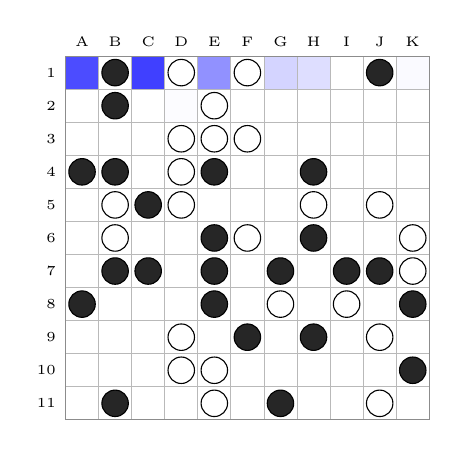
\begin{tikzpicture}[x=0.42cm, y=0.42cm]
\fill[blue!70] (0,0) rectangle (1,-1);
\fill[blue!75] (2,0) rectangle (3,-1);
\fill[blue!43] (4,0) rectangle (5,-1);
\fill[blue!17] (6,0) rectangle (7,-1);
\fill[blue!13] (7,0) rectangle (8,-1);
\fill[blue!2] (10,0) rectangle (11,-1);
\fill[blue!1] (3,-1) rectangle (4,-2);
\draw[gray!55, line width=.3pt, step=1] (0,0) grid (11,-11);
\draw[gray!90] (0,0) rectangle (11,-11);
\node[font=\tiny, anchor=south] at (0.5,0) {A};
\node[font=\tiny, anchor=south] at (1.5,0) {B};
\node[font=\tiny, anchor=south] at (2.5,0) {C};
\node[font=\tiny, anchor=south] at (3.5,0) {D};
\node[font=\tiny, anchor=south] at (4.5,0) {E};
\node[font=\tiny, anchor=south] at (5.5,0) {F};
\node[font=\tiny, anchor=south] at (6.5,0) {G};
\node[font=\tiny, anchor=south] at (7.5,0) {H};
\node[font=\tiny, anchor=south] at (8.5,0) {I};
\node[font=\tiny, anchor=south] at (9.5,0) {J};
\node[font=\tiny, anchor=south] at (10.5,0) {K};
\node[font=\tiny, anchor=east] at (0,-0.5) {1};
\node[font=\tiny, anchor=east] at (0,-1.5) {2};
\node[font=\tiny, anchor=east] at (0,-2.5) {3};
\node[font=\tiny, anchor=east] at (0,-3.5) {4};
\node[font=\tiny, anchor=east] at (0,-4.5) {5};
\node[font=\tiny, anchor=east] at (0,-5.5) {6};
\node[font=\tiny, anchor=east] at (0,-6.5) {7};
\node[font=\tiny, anchor=east] at (0,-7.5) {8};
\node[font=\tiny, anchor=east] at (0,-8.5) {9};
\node[font=\tiny, anchor=east] at (0,-9.5) {10};
\node[font=\tiny, anchor=east] at (0,-10.5) {11};
\draw[fill=black!85, line width=.4pt] (1.5,-0.5) circle (.40);
\draw[fill=white, line width=.4pt] (3.5,-0.5) circle (.40);
\draw[fill=white, line width=.4pt] (5.5,-0.5) circle (.40);
\draw[fill=black!85, line width=.4pt] (9.5,-0.5) circle (.40);
\draw[fill=black!85, line width=.4pt] (1.5,-1.5) circle (.40);
\draw[fill=white, line width=.4pt] (4.5,-1.5) circle (.40);
\draw[fill=white, line width=.4pt] (3.5,-2.5) circle (.40);
\draw[fill=white, line width=.4pt] (4.5,-2.5) circle (.40);
\draw[fill=white, line width=.4pt] (5.5,-2.5) circle (.40);
\draw[fill=black!85, line width=.4pt] (0.5,-3.5) circle (.40);
\draw[fill=black!85, line width=.4pt] (1.5,-3.5) circle (.40);
\draw[fill=white, line width=.4pt] (3.5,-3.5) circle (.40);
\draw[fill=black!85, line width=.4pt] (4.5,-3.5) circle (.40);
\draw[fill=black!85, line width=.4pt] (7.5,-3.5) circle (.40);
\draw[fill=white, line width=.4pt] (1.5,-4.5) circle (.40);
\draw[fill=black!85, line width=.4pt] (2.5,-4.5) circle (.40);
\draw[fill=white, line width=.4pt] (3.5,-4.5) circle (.40);
\draw[fill=white, line width=.4pt] (7.5,-4.5) circle (.40);
\draw[fill=white, line width=.4pt] (9.5,-4.5) circle (.40);
\draw[fill=white, line width=.4pt] (1.5,-5.5) circle (.40);
\draw[fill=black!85, line width=.4pt] (4.5,-5.5) circle (.40);
\draw[fill=white, line width=.4pt] (5.5,-5.5) circle (.40);
\draw[fill=black!85, line width=.4pt] (7.5,-5.5) circle (.40);
\draw[fill=white, line width=.4pt] (10.5,-5.5) circle (.40);
\draw[fill=black!85, line width=.4pt] (1.5,-6.5) circle (.40);
\draw[fill=black!85, line width=.4pt] (2.5,-6.5) circle (.40);
\draw[fill=black!85, line width=.4pt] (4.5,-6.5) circle (.40);
\draw[fill=black!85, line width=.4pt] (6.5,-6.5) circle (.40);
\draw[fill=black!85, line width=.4pt] (8.5,-6.5) circle (.40);
\draw[fill=black!85, line width=.4pt] (9.5,-6.5) circle (.40);
\draw[fill=white, line width=.4pt] (10.5,-6.5) circle (.40);
\draw[fill=black!85, line width=.4pt] (0.5,-7.5) circle (.40);
\draw[fill=black!85, line width=.4pt] (4.5,-7.5) circle (.40);
\draw[fill=white, line width=.4pt] (6.5,-7.5) circle (.40);
\draw[fill=white, line width=.4pt] (8.5,-7.5) circle (.40);
\draw[fill=black!85, line width=.4pt] (10.5,-7.5) circle (.40);
\draw[fill=white, line width=.4pt] (3.5,-8.5) circle (.40);
\draw[fill=black!85, line width=.4pt] (5.5,-8.5) circle (.40);
\draw[fill=black!85, line width=.4pt] (7.5,-8.5) circle (.40);
\draw[fill=white, line width=.4pt] (9.5,-8.5) circle (.40);
\draw[fill=white, line width=.4pt] (3.5,-9.5) circle (.40);
\draw[fill=white, line width=.4pt] (4.5,-9.5) circle (.40);
\draw[fill=black!85, line width=.4pt] (10.5,-9.5) circle (.40);
\draw[fill=black!85, line width=.4pt] (1.5,-10.5) circle (.40);
\draw[fill=white, line width=.4pt] (4.5,-10.5) circle (.40);
\draw[fill=black!85, line width=.4pt] (6.5,-10.5) circle (.40);
\draw[fill=white, line width=.4pt] (9.5,-10.5) circle (.40);
\end{tikzpicture}
    \caption{SL không aug: $v=0{,}38$; đáp án 1,0\%; cao nhất C1 (33,5\%)}
  \end{subfigure}\par\medskip
  \begin{subfigure}[t]{.48\linewidth}
    \centering
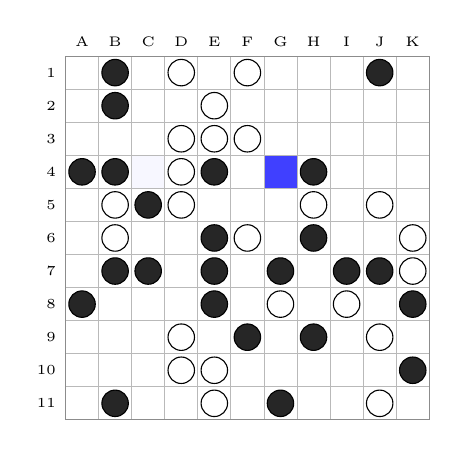
\begin{tikzpicture}[x=0.42cm, y=0.42cm]
\fill[blue!3] (2,-3) rectangle (3,-4);
\fill[blue!75] (6,-3) rectangle (7,-4);
\draw[gray!55, line width=.3pt, step=1] (0,0) grid (11,-11);
\draw[gray!90] (0,0) rectangle (11,-11);
\node[font=\tiny, anchor=south] at (0.5,0) {A};
\node[font=\tiny, anchor=south] at (1.5,0) {B};
\node[font=\tiny, anchor=south] at (2.5,0) {C};
\node[font=\tiny, anchor=south] at (3.5,0) {D};
\node[font=\tiny, anchor=south] at (4.5,0) {E};
\node[font=\tiny, anchor=south] at (5.5,0) {F};
\node[font=\tiny, anchor=south] at (6.5,0) {G};
\node[font=\tiny, anchor=south] at (7.5,0) {H};
\node[font=\tiny, anchor=south] at (8.5,0) {I};
\node[font=\tiny, anchor=south] at (9.5,0) {J};
\node[font=\tiny, anchor=south] at (10.5,0) {K};
\node[font=\tiny, anchor=east] at (0,-0.5) {1};
\node[font=\tiny, anchor=east] at (0,-1.5) {2};
\node[font=\tiny, anchor=east] at (0,-2.5) {3};
\node[font=\tiny, anchor=east] at (0,-3.5) {4};
\node[font=\tiny, anchor=east] at (0,-4.5) {5};
\node[font=\tiny, anchor=east] at (0,-5.5) {6};
\node[font=\tiny, anchor=east] at (0,-6.5) {7};
\node[font=\tiny, anchor=east] at (0,-7.5) {8};
\node[font=\tiny, anchor=east] at (0,-8.5) {9};
\node[font=\tiny, anchor=east] at (0,-9.5) {10};
\node[font=\tiny, anchor=east] at (0,-10.5) {11};
\draw[fill=black!85, line width=.4pt] (1.5,-0.5) circle (.40);
\draw[fill=white, line width=.4pt] (3.5,-0.5) circle (.40);
\draw[fill=white, line width=.4pt] (5.5,-0.5) circle (.40);
\draw[fill=black!85, line width=.4pt] (9.5,-0.5) circle (.40);
\draw[fill=black!85, line width=.4pt] (1.5,-1.5) circle (.40);
\draw[fill=white, line width=.4pt] (4.5,-1.5) circle (.40);
\draw[fill=white, line width=.4pt] (3.5,-2.5) circle (.40);
\draw[fill=white, line width=.4pt] (4.5,-2.5) circle (.40);
\draw[fill=white, line width=.4pt] (5.5,-2.5) circle (.40);
\draw[fill=black!85, line width=.4pt] (0.5,-3.5) circle (.40);
\draw[fill=black!85, line width=.4pt] (1.5,-3.5) circle (.40);
\draw[fill=white, line width=.4pt] (3.5,-3.5) circle (.40);
\draw[fill=black!85, line width=.4pt] (4.5,-3.5) circle (.40);
\draw[fill=black!85, line width=.4pt] (7.5,-3.5) circle (.40);
\draw[fill=white, line width=.4pt] (1.5,-4.5) circle (.40);
\draw[fill=black!85, line width=.4pt] (2.5,-4.5) circle (.40);
\draw[fill=white, line width=.4pt] (3.5,-4.5) circle (.40);
\draw[fill=white, line width=.4pt] (7.5,-4.5) circle (.40);
\draw[fill=white, line width=.4pt] (9.5,-4.5) circle (.40);
\draw[fill=white, line width=.4pt] (1.5,-5.5) circle (.40);
\draw[fill=black!85, line width=.4pt] (4.5,-5.5) circle (.40);
\draw[fill=white, line width=.4pt] (5.5,-5.5) circle (.40);
\draw[fill=black!85, line width=.4pt] (7.5,-5.5) circle (.40);
\draw[fill=white, line width=.4pt] (10.5,-5.5) circle (.40);
\draw[fill=black!85, line width=.4pt] (1.5,-6.5) circle (.40);
\draw[fill=black!85, line width=.4pt] (2.5,-6.5) circle (.40);
\draw[fill=black!85, line width=.4pt] (4.5,-6.5) circle (.40);
\draw[fill=black!85, line width=.4pt] (6.5,-6.5) circle (.40);
\draw[fill=black!85, line width=.4pt] (8.5,-6.5) circle (.40);
\draw[fill=black!85, line width=.4pt] (9.5,-6.5) circle (.40);
\draw[fill=white, line width=.4pt] (10.5,-6.5) circle (.40);
\draw[fill=black!85, line width=.4pt] (0.5,-7.5) circle (.40);
\draw[fill=black!85, line width=.4pt] (4.5,-7.5) circle (.40);
\draw[fill=white, line width=.4pt] (6.5,-7.5) circle (.40);
\draw[fill=white, line width=.4pt] (8.5,-7.5) circle (.40);
\draw[fill=black!85, line width=.4pt] (10.5,-7.5) circle (.40);
\draw[fill=white, line width=.4pt] (3.5,-8.5) circle (.40);
\draw[fill=black!85, line width=.4pt] (5.5,-8.5) circle (.40);
\draw[fill=black!85, line width=.4pt] (7.5,-8.5) circle (.40);
\draw[fill=white, line width=.4pt] (9.5,-8.5) circle (.40);
\draw[fill=white, line width=.4pt] (3.5,-9.5) circle (.40);
\draw[fill=white, line width=.4pt] (4.5,-9.5) circle (.40);
\draw[fill=black!85, line width=.4pt] (10.5,-9.5) circle (.40);
\draw[fill=black!85, line width=.4pt] (1.5,-10.5) circle (.40);
\draw[fill=white, line width=.4pt] (4.5,-10.5) circle (.40);
\draw[fill=black!85, line width=.4pt] (6.5,-10.5) circle (.40);
\draw[fill=white, line width=.4pt] (9.5,-10.5) circle (.40);
\end{tikzpicture}
    \caption{L6 (RL): $v=1{,}00$; đáp án 99,6\%; cao nhất G4 (95,9\%)}
  \end{subfigure}\hfill
  \begin{subfigure}[t]{.48\linewidth}
    \centering
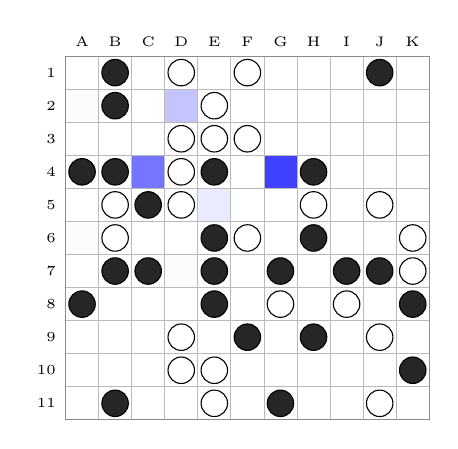
\begin{tikzpicture}[x=0.42cm, y=0.42cm]
\fill[blue!1] (0,-1) rectangle (1,-2);
\fill[blue!23] (3,-1) rectangle (4,-2);
\fill[blue!54] (2,-3) rectangle (3,-4);
\fill[blue!75] (6,-3) rectangle (7,-4);
\fill[blue!8] (4,-4) rectangle (5,-5);
\fill[blue!1] (0,-5) rectangle (1,-6);
\fill[blue!1] (3,-6) rectangle (4,-7);
\draw[gray!55, line width=.3pt, step=1] (0,0) grid (11,-11);
\draw[gray!90] (0,0) rectangle (11,-11);
\node[font=\tiny, anchor=south] at (0.5,0) {A};
\node[font=\tiny, anchor=south] at (1.5,0) {B};
\node[font=\tiny, anchor=south] at (2.5,0) {C};
\node[font=\tiny, anchor=south] at (3.5,0) {D};
\node[font=\tiny, anchor=south] at (4.5,0) {E};
\node[font=\tiny, anchor=south] at (5.5,0) {F};
\node[font=\tiny, anchor=south] at (6.5,0) {G};
\node[font=\tiny, anchor=south] at (7.5,0) {H};
\node[font=\tiny, anchor=south] at (8.5,0) {I};
\node[font=\tiny, anchor=south] at (9.5,0) {J};
\node[font=\tiny, anchor=south] at (10.5,0) {K};
\node[font=\tiny, anchor=east] at (0,-0.5) {1};
\node[font=\tiny, anchor=east] at (0,-1.5) {2};
\node[font=\tiny, anchor=east] at (0,-2.5) {3};
\node[font=\tiny, anchor=east] at (0,-3.5) {4};
\node[font=\tiny, anchor=east] at (0,-4.5) {5};
\node[font=\tiny, anchor=east] at (0,-5.5) {6};
\node[font=\tiny, anchor=east] at (0,-6.5) {7};
\node[font=\tiny, anchor=east] at (0,-7.5) {8};
\node[font=\tiny, anchor=east] at (0,-8.5) {9};
\node[font=\tiny, anchor=east] at (0,-9.5) {10};
\node[font=\tiny, anchor=east] at (0,-10.5) {11};
\draw[fill=black!85, line width=.4pt] (1.5,-0.5) circle (.40);
\draw[fill=white, line width=.4pt] (3.5,-0.5) circle (.40);
\draw[fill=white, line width=.4pt] (5.5,-0.5) circle (.40);
\draw[fill=black!85, line width=.4pt] (9.5,-0.5) circle (.40);
\draw[fill=black!85, line width=.4pt] (1.5,-1.5) circle (.40);
\draw[fill=white, line width=.4pt] (4.5,-1.5) circle (.40);
\draw[fill=white, line width=.4pt] (3.5,-2.5) circle (.40);
\draw[fill=white, line width=.4pt] (4.5,-2.5) circle (.40);
\draw[fill=white, line width=.4pt] (5.5,-2.5) circle (.40);
\draw[fill=black!85, line width=.4pt] (0.5,-3.5) circle (.40);
\draw[fill=black!85, line width=.4pt] (1.5,-3.5) circle (.40);
\draw[fill=white, line width=.4pt] (3.5,-3.5) circle (.40);
\draw[fill=black!85, line width=.4pt] (4.5,-3.5) circle (.40);
\draw[fill=black!85, line width=.4pt] (7.5,-3.5) circle (.40);
\draw[fill=white, line width=.4pt] (1.5,-4.5) circle (.40);
\draw[fill=black!85, line width=.4pt] (2.5,-4.5) circle (.40);
\draw[fill=white, line width=.4pt] (3.5,-4.5) circle (.40);
\draw[fill=white, line width=.4pt] (7.5,-4.5) circle (.40);
\draw[fill=white, line width=.4pt] (9.5,-4.5) circle (.40);
\draw[fill=white, line width=.4pt] (1.5,-5.5) circle (.40);
\draw[fill=black!85, line width=.4pt] (4.5,-5.5) circle (.40);
\draw[fill=white, line width=.4pt] (5.5,-5.5) circle (.40);
\draw[fill=black!85, line width=.4pt] (7.5,-5.5) circle (.40);
\draw[fill=white, line width=.4pt] (10.5,-5.5) circle (.40);
\draw[fill=black!85, line width=.4pt] (1.5,-6.5) circle (.40);
\draw[fill=black!85, line width=.4pt] (2.5,-6.5) circle (.40);
\draw[fill=black!85, line width=.4pt] (4.5,-6.5) circle (.40);
\draw[fill=black!85, line width=.4pt] (6.5,-6.5) circle (.40);
\draw[fill=black!85, line width=.4pt] (8.5,-6.5) circle (.40);
\draw[fill=black!85, line width=.4pt] (9.5,-6.5) circle (.40);
\draw[fill=white, line width=.4pt] (10.5,-6.5) circle (.40);
\draw[fill=black!85, line width=.4pt] (0.5,-7.5) circle (.40);
\draw[fill=black!85, line width=.4pt] (4.5,-7.5) circle (.40);
\draw[fill=white, line width=.4pt] (6.5,-7.5) circle (.40);
\draw[fill=white, line width=.4pt] (8.5,-7.5) circle (.40);
\draw[fill=black!85, line width=.4pt] (10.5,-7.5) circle (.40);
\draw[fill=white, line width=.4pt] (3.5,-8.5) circle (.40);
\draw[fill=black!85, line width=.4pt] (5.5,-8.5) circle (.40);
\draw[fill=black!85, line width=.4pt] (7.5,-8.5) circle (.40);
\draw[fill=white, line width=.4pt] (9.5,-8.5) circle (.40);
\draw[fill=white, line width=.4pt] (3.5,-9.5) circle (.40);
\draw[fill=white, line width=.4pt] (4.5,-9.5) circle (.40);
\draw[fill=black!85, line width=.4pt] (10.5,-9.5) circle (.40);
\draw[fill=black!85, line width=.4pt] (1.5,-10.5) circle (.40);
\draw[fill=white, line width=.4pt] (4.5,-10.5) circle (.40);
\draw[fill=black!85, line width=.4pt] (6.5,-10.5) circle (.40);
\draw[fill=white, line width=.4pt] (9.5,-10.5) circle (.40);
\end{tikzpicture}
    \caption{L8 (AZ): $v=1{,}00$; đáp án 86,0\%; cao nhất G4 (42,5\%)}
  \end{subfigure}\par\medskip
  \caption{Policy của bốn mạng tại thế C1-001 (O đi). Ô càng đậm xác suất càng cao (chuẩn hoá theo ô lớn nhất của từng mạng). Đáp án: D2, C4, G4.}
  \label{fig:cs-policy-c1}
\end{figure}

\begin{figure}[H]
  \centering
  \begin{subfigure}[t]{.48\linewidth}
    \centering
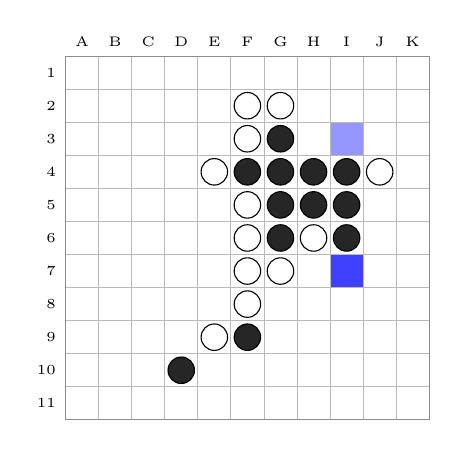
\begin{tikzpicture}[x=0.42cm, y=0.42cm]
\fill[blue!41] (8,-2) rectangle (9,-3);
\fill[blue!75] (8,-6) rectangle (9,-7);
\draw[gray!55, line width=.3pt, step=1] (0,0) grid (11,-11);
\draw[gray!90] (0,0) rectangle (11,-11);
\node[font=\tiny, anchor=south] at (0.5,0) {A};
\node[font=\tiny, anchor=south] at (1.5,0) {B};
\node[font=\tiny, anchor=south] at (2.5,0) {C};
\node[font=\tiny, anchor=south] at (3.5,0) {D};
\node[font=\tiny, anchor=south] at (4.5,0) {E};
\node[font=\tiny, anchor=south] at (5.5,0) {F};
\node[font=\tiny, anchor=south] at (6.5,0) {G};
\node[font=\tiny, anchor=south] at (7.5,0) {H};
\node[font=\tiny, anchor=south] at (8.5,0) {I};
\node[font=\tiny, anchor=south] at (9.5,0) {J};
\node[font=\tiny, anchor=south] at (10.5,0) {K};
\node[font=\tiny, anchor=east] at (0,-0.5) {1};
\node[font=\tiny, anchor=east] at (0,-1.5) {2};
\node[font=\tiny, anchor=east] at (0,-2.5) {3};
\node[font=\tiny, anchor=east] at (0,-3.5) {4};
\node[font=\tiny, anchor=east] at (0,-4.5) {5};
\node[font=\tiny, anchor=east] at (0,-5.5) {6};
\node[font=\tiny, anchor=east] at (0,-6.5) {7};
\node[font=\tiny, anchor=east] at (0,-7.5) {8};
\node[font=\tiny, anchor=east] at (0,-8.5) {9};
\node[font=\tiny, anchor=east] at (0,-9.5) {10};
\node[font=\tiny, anchor=east] at (0,-10.5) {11};
\draw[fill=white, line width=.4pt] (5.5,-1.5) circle (.40);
\draw[fill=white, line width=.4pt] (6.5,-1.5) circle (.40);
\draw[fill=white, line width=.4pt] (5.5,-2.5) circle (.40);
\draw[fill=black!85, line width=.4pt] (6.5,-2.5) circle (.40);
\draw[fill=white, line width=.4pt] (4.5,-3.5) circle (.40);
\draw[fill=black!85, line width=.4pt] (5.5,-3.5) circle (.40);
\draw[fill=black!85, line width=.4pt] (6.5,-3.5) circle (.40);
\draw[fill=black!85, line width=.4pt] (7.5,-3.5) circle (.40);
\draw[fill=black!85, line width=.4pt] (8.5,-3.5) circle (.40);
\draw[fill=white, line width=.4pt] (9.5,-3.5) circle (.40);
\draw[fill=white, line width=.4pt] (5.5,-4.5) circle (.40);
\draw[fill=black!85, line width=.4pt] (6.5,-4.5) circle (.40);
\draw[fill=black!85, line width=.4pt] (7.5,-4.5) circle (.40);
\draw[fill=black!85, line width=.4pt] (8.5,-4.5) circle (.40);
\draw[fill=white, line width=.4pt] (5.5,-5.5) circle (.40);
\draw[fill=black!85, line width=.4pt] (6.5,-5.5) circle (.40);
\draw[fill=white, line width=.4pt] (7.5,-5.5) circle (.40);
\draw[fill=black!85, line width=.4pt] (8.5,-5.5) circle (.40);
\draw[fill=white, line width=.4pt] (5.5,-6.5) circle (.40);
\draw[fill=white, line width=.4pt] (6.5,-6.5) circle (.40);
\draw[fill=white, line width=.4pt] (5.5,-7.5) circle (.40);
\draw[fill=white, line width=.4pt] (4.5,-8.5) circle (.40);
\draw[fill=black!85, line width=.4pt] (5.5,-8.5) circle (.40);
\draw[fill=black!85, line width=.4pt] (3.5,-9.5) circle (.40);
\end{tikzpicture}
    \caption{SL v3: $v=0{,}99$; đáp án 99,9\%; cao nhất I7 (64,1\%)}
  \end{subfigure}\hfill
  \begin{subfigure}[t]{.48\linewidth}
    \centering
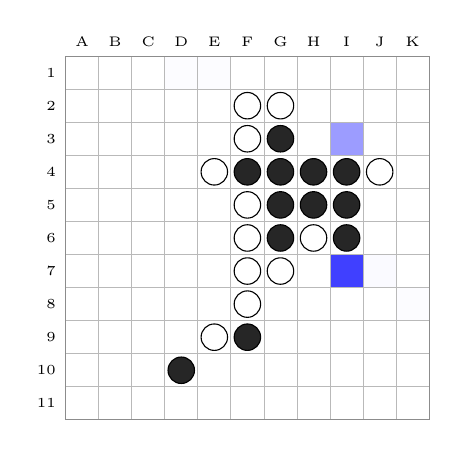
\begin{tikzpicture}[x=0.42cm, y=0.42cm]
\fill[blue!1] (3,0) rectangle (4,-1);
\fill[blue!1] (4,0) rectangle (5,-1);
\fill[blue!39] (8,-2) rectangle (9,-3);
\fill[blue!75] (8,-6) rectangle (9,-7);
\fill[blue!2] (9,-6) rectangle (10,-7);
\fill[blue!1] (10,-7) rectangle (11,-8);
\draw[gray!55, line width=.3pt, step=1] (0,0) grid (11,-11);
\draw[gray!90] (0,0) rectangle (11,-11);
\node[font=\tiny, anchor=south] at (0.5,0) {A};
\node[font=\tiny, anchor=south] at (1.5,0) {B};
\node[font=\tiny, anchor=south] at (2.5,0) {C};
\node[font=\tiny, anchor=south] at (3.5,0) {D};
\node[font=\tiny, anchor=south] at (4.5,0) {E};
\node[font=\tiny, anchor=south] at (5.5,0) {F};
\node[font=\tiny, anchor=south] at (6.5,0) {G};
\node[font=\tiny, anchor=south] at (7.5,0) {H};
\node[font=\tiny, anchor=south] at (8.5,0) {I};
\node[font=\tiny, anchor=south] at (9.5,0) {J};
\node[font=\tiny, anchor=south] at (10.5,0) {K};
\node[font=\tiny, anchor=east] at (0,-0.5) {1};
\node[font=\tiny, anchor=east] at (0,-1.5) {2};
\node[font=\tiny, anchor=east] at (0,-2.5) {3};
\node[font=\tiny, anchor=east] at (0,-3.5) {4};
\node[font=\tiny, anchor=east] at (0,-4.5) {5};
\node[font=\tiny, anchor=east] at (0,-5.5) {6};
\node[font=\tiny, anchor=east] at (0,-6.5) {7};
\node[font=\tiny, anchor=east] at (0,-7.5) {8};
\node[font=\tiny, anchor=east] at (0,-8.5) {9};
\node[font=\tiny, anchor=east] at (0,-9.5) {10};
\node[font=\tiny, anchor=east] at (0,-10.5) {11};
\draw[fill=white, line width=.4pt] (5.5,-1.5) circle (.40);
\draw[fill=white, line width=.4pt] (6.5,-1.5) circle (.40);
\draw[fill=white, line width=.4pt] (5.5,-2.5) circle (.40);
\draw[fill=black!85, line width=.4pt] (6.5,-2.5) circle (.40);
\draw[fill=white, line width=.4pt] (4.5,-3.5) circle (.40);
\draw[fill=black!85, line width=.4pt] (5.5,-3.5) circle (.40);
\draw[fill=black!85, line width=.4pt] (6.5,-3.5) circle (.40);
\draw[fill=black!85, line width=.4pt] (7.5,-3.5) circle (.40);
\draw[fill=black!85, line width=.4pt] (8.5,-3.5) circle (.40);
\draw[fill=white, line width=.4pt] (9.5,-3.5) circle (.40);
\draw[fill=white, line width=.4pt] (5.5,-4.5) circle (.40);
\draw[fill=black!85, line width=.4pt] (6.5,-4.5) circle (.40);
\draw[fill=black!85, line width=.4pt] (7.5,-4.5) circle (.40);
\draw[fill=black!85, line width=.4pt] (8.5,-4.5) circle (.40);
\draw[fill=white, line width=.4pt] (5.5,-5.5) circle (.40);
\draw[fill=black!85, line width=.4pt] (6.5,-5.5) circle (.40);
\draw[fill=white, line width=.4pt] (7.5,-5.5) circle (.40);
\draw[fill=black!85, line width=.4pt] (8.5,-5.5) circle (.40);
\draw[fill=white, line width=.4pt] (5.5,-6.5) circle (.40);
\draw[fill=white, line width=.4pt] (6.5,-6.5) circle (.40);
\draw[fill=white, line width=.4pt] (5.5,-7.5) circle (.40);
\draw[fill=white, line width=.4pt] (4.5,-8.5) circle (.40);
\draw[fill=black!85, line width=.4pt] (5.5,-8.5) circle (.40);
\draw[fill=black!85, line width=.4pt] (3.5,-9.5) circle (.40);
\end{tikzpicture}
    \caption{SL không aug: $v=0{,}97$; đáp án 96,8\%; cao nhất I7 (60,6\%)}
  \end{subfigure}\par\medskip
  \begin{subfigure}[t]{.48\linewidth}
    \centering
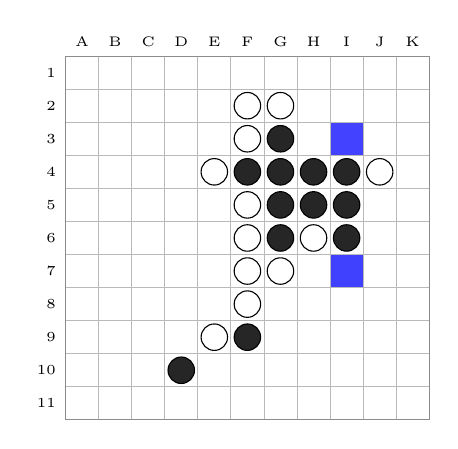
\begin{tikzpicture}[x=0.42cm, y=0.42cm]
\fill[blue!74] (8,-2) rectangle (9,-3);
\fill[blue!75] (8,-6) rectangle (9,-7);
\draw[gray!55, line width=.3pt, step=1] (0,0) grid (11,-11);
\draw[gray!90] (0,0) rectangle (11,-11);
\node[font=\tiny, anchor=south] at (0.5,0) {A};
\node[font=\tiny, anchor=south] at (1.5,0) {B};
\node[font=\tiny, anchor=south] at (2.5,0) {C};
\node[font=\tiny, anchor=south] at (3.5,0) {D};
\node[font=\tiny, anchor=south] at (4.5,0) {E};
\node[font=\tiny, anchor=south] at (5.5,0) {F};
\node[font=\tiny, anchor=south] at (6.5,0) {G};
\node[font=\tiny, anchor=south] at (7.5,0) {H};
\node[font=\tiny, anchor=south] at (8.5,0) {I};
\node[font=\tiny, anchor=south] at (9.5,0) {J};
\node[font=\tiny, anchor=south] at (10.5,0) {K};
\node[font=\tiny, anchor=east] at (0,-0.5) {1};
\node[font=\tiny, anchor=east] at (0,-1.5) {2};
\node[font=\tiny, anchor=east] at (0,-2.5) {3};
\node[font=\tiny, anchor=east] at (0,-3.5) {4};
\node[font=\tiny, anchor=east] at (0,-4.5) {5};
\node[font=\tiny, anchor=east] at (0,-5.5) {6};
\node[font=\tiny, anchor=east] at (0,-6.5) {7};
\node[font=\tiny, anchor=east] at (0,-7.5) {8};
\node[font=\tiny, anchor=east] at (0,-8.5) {9};
\node[font=\tiny, anchor=east] at (0,-9.5) {10};
\node[font=\tiny, anchor=east] at (0,-10.5) {11};
\draw[fill=white, line width=.4pt] (5.5,-1.5) circle (.40);
\draw[fill=white, line width=.4pt] (6.5,-1.5) circle (.40);
\draw[fill=white, line width=.4pt] (5.5,-2.5) circle (.40);
\draw[fill=black!85, line width=.4pt] (6.5,-2.5) circle (.40);
\draw[fill=white, line width=.4pt] (4.5,-3.5) circle (.40);
\draw[fill=black!85, line width=.4pt] (5.5,-3.5) circle (.40);
\draw[fill=black!85, line width=.4pt] (6.5,-3.5) circle (.40);
\draw[fill=black!85, line width=.4pt] (7.5,-3.5) circle (.40);
\draw[fill=black!85, line width=.4pt] (8.5,-3.5) circle (.40);
\draw[fill=white, line width=.4pt] (9.5,-3.5) circle (.40);
\draw[fill=white, line width=.4pt] (5.5,-4.5) circle (.40);
\draw[fill=black!85, line width=.4pt] (6.5,-4.5) circle (.40);
\draw[fill=black!85, line width=.4pt] (7.5,-4.5) circle (.40);
\draw[fill=black!85, line width=.4pt] (8.5,-4.5) circle (.40);
\draw[fill=white, line width=.4pt] (5.5,-5.5) circle (.40);
\draw[fill=black!85, line width=.4pt] (6.5,-5.5) circle (.40);
\draw[fill=white, line width=.4pt] (7.5,-5.5) circle (.40);
\draw[fill=black!85, line width=.4pt] (8.5,-5.5) circle (.40);
\draw[fill=white, line width=.4pt] (5.5,-6.5) circle (.40);
\draw[fill=white, line width=.4pt] (6.5,-6.5) circle (.40);
\draw[fill=white, line width=.4pt] (5.5,-7.5) circle (.40);
\draw[fill=white, line width=.4pt] (4.5,-8.5) circle (.40);
\draw[fill=black!85, line width=.4pt] (5.5,-8.5) circle (.40);
\draw[fill=black!85, line width=.4pt] (3.5,-9.5) circle (.40);
\end{tikzpicture}
    \caption{L6 (RL): $v=0{,}84$; đáp án 100,0\%; cao nhất I7 (50,2\%)}
  \end{subfigure}\hfill
  \begin{subfigure}[t]{.48\linewidth}
    \centering
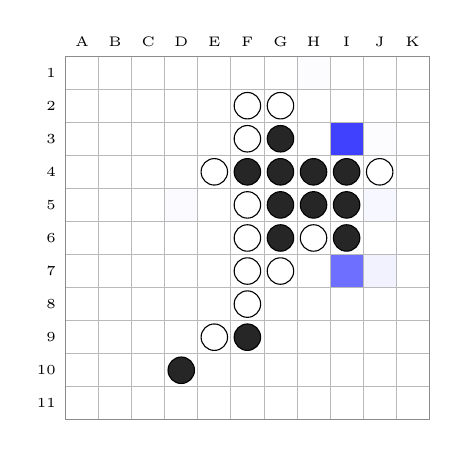
\begin{tikzpicture}[x=0.42cm, y=0.42cm]
\fill[blue!1] (7,0) rectangle (8,-1);
\fill[blue!75] (8,-2) rectangle (9,-3);
\fill[blue!1] (9,-2) rectangle (10,-3);
\fill[blue!2] (3,-4) rectangle (4,-5);
\fill[blue!3] (9,-4) rectangle (10,-5);
\fill[blue!57] (8,-6) rectangle (9,-7);
\fill[blue!5] (9,-6) rectangle (10,-7);
\draw[gray!55, line width=.3pt, step=1] (0,0) grid (11,-11);
\draw[gray!90] (0,0) rectangle (11,-11);
\node[font=\tiny, anchor=south] at (0.5,0) {A};
\node[font=\tiny, anchor=south] at (1.5,0) {B};
\node[font=\tiny, anchor=south] at (2.5,0) {C};
\node[font=\tiny, anchor=south] at (3.5,0) {D};
\node[font=\tiny, anchor=south] at (4.5,0) {E};
\node[font=\tiny, anchor=south] at (5.5,0) {F};
\node[font=\tiny, anchor=south] at (6.5,0) {G};
\node[font=\tiny, anchor=south] at (7.5,0) {H};
\node[font=\tiny, anchor=south] at (8.5,0) {I};
\node[font=\tiny, anchor=south] at (9.5,0) {J};
\node[font=\tiny, anchor=south] at (10.5,0) {K};
\node[font=\tiny, anchor=east] at (0,-0.5) {1};
\node[font=\tiny, anchor=east] at (0,-1.5) {2};
\node[font=\tiny, anchor=east] at (0,-2.5) {3};
\node[font=\tiny, anchor=east] at (0,-3.5) {4};
\node[font=\tiny, anchor=east] at (0,-4.5) {5};
\node[font=\tiny, anchor=east] at (0,-5.5) {6};
\node[font=\tiny, anchor=east] at (0,-6.5) {7};
\node[font=\tiny, anchor=east] at (0,-7.5) {8};
\node[font=\tiny, anchor=east] at (0,-8.5) {9};
\node[font=\tiny, anchor=east] at (0,-9.5) {10};
\node[font=\tiny, anchor=east] at (0,-10.5) {11};
\draw[fill=white, line width=.4pt] (5.5,-1.5) circle (.40);
\draw[fill=white, line width=.4pt] (6.5,-1.5) circle (.40);
\draw[fill=white, line width=.4pt] (5.5,-2.5) circle (.40);
\draw[fill=black!85, line width=.4pt] (6.5,-2.5) circle (.40);
\draw[fill=white, line width=.4pt] (4.5,-3.5) circle (.40);
\draw[fill=black!85, line width=.4pt] (5.5,-3.5) circle (.40);
\draw[fill=black!85, line width=.4pt] (6.5,-3.5) circle (.40);
\draw[fill=black!85, line width=.4pt] (7.5,-3.5) circle (.40);
\draw[fill=black!85, line width=.4pt] (8.5,-3.5) circle (.40);
\draw[fill=white, line width=.4pt] (9.5,-3.5) circle (.40);
\draw[fill=white, line width=.4pt] (5.5,-4.5) circle (.40);
\draw[fill=black!85, line width=.4pt] (6.5,-4.5) circle (.40);
\draw[fill=black!85, line width=.4pt] (7.5,-4.5) circle (.40);
\draw[fill=black!85, line width=.4pt] (8.5,-4.5) circle (.40);
\draw[fill=white, line width=.4pt] (5.5,-5.5) circle (.40);
\draw[fill=black!85, line width=.4pt] (6.5,-5.5) circle (.40);
\draw[fill=white, line width=.4pt] (7.5,-5.5) circle (.40);
\draw[fill=black!85, line width=.4pt] (8.5,-5.5) circle (.40);
\draw[fill=white, line width=.4pt] (5.5,-6.5) circle (.40);
\draw[fill=white, line width=.4pt] (6.5,-6.5) circle (.40);
\draw[fill=white, line width=.4pt] (5.5,-7.5) circle (.40);
\draw[fill=white, line width=.4pt] (4.5,-8.5) circle (.40);
\draw[fill=black!85, line width=.4pt] (5.5,-8.5) circle (.40);
\draw[fill=black!85, line width=.4pt] (3.5,-9.5) circle (.40);
\end{tikzpicture}
    \caption{L8 (AZ): $v=0{,}98$; đáp án 96,4\%; cao nhất I3 (50,6\%)}
  \end{subfigure}\par\medskip
  \caption{Policy của bốn mạng tại thế C3-001 (X đi). Ô càng đậm xác suất càng cao (chuẩn hoá theo ô lớn nhất của từng mạng). Đáp án: I2, K2, I3, J3, J5, K5.}
  \label{fig:cs-policy-c3}
\end{figure}

\begin{figure}[H]
  \centering
  \begin{subfigure}[t]{.48\linewidth}
    \centering
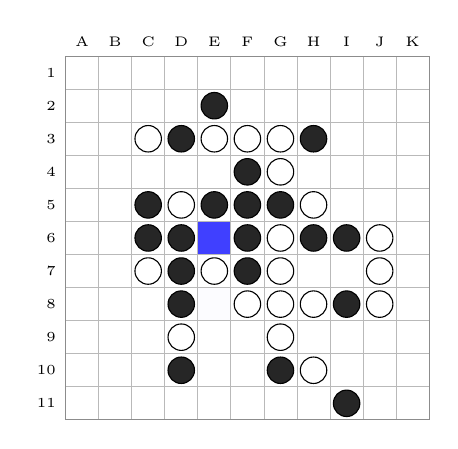
\begin{tikzpicture}[x=0.42cm, y=0.42cm]
\fill[blue!75] (4,-5) rectangle (5,-6);
\fill[blue!1] (4,-7) rectangle (5,-8);
\draw[gray!55, line width=.3pt, step=1] (0,0) grid (11,-11);
\draw[gray!90] (0,0) rectangle (11,-11);
\node[font=\tiny, anchor=south] at (0.5,0) {A};
\node[font=\tiny, anchor=south] at (1.5,0) {B};
\node[font=\tiny, anchor=south] at (2.5,0) {C};
\node[font=\tiny, anchor=south] at (3.5,0) {D};
\node[font=\tiny, anchor=south] at (4.5,0) {E};
\node[font=\tiny, anchor=south] at (5.5,0) {F};
\node[font=\tiny, anchor=south] at (6.5,0) {G};
\node[font=\tiny, anchor=south] at (7.5,0) {H};
\node[font=\tiny, anchor=south] at (8.5,0) {I};
\node[font=\tiny, anchor=south] at (9.5,0) {J};
\node[font=\tiny, anchor=south] at (10.5,0) {K};
\node[font=\tiny, anchor=east] at (0,-0.5) {1};
\node[font=\tiny, anchor=east] at (0,-1.5) {2};
\node[font=\tiny, anchor=east] at (0,-2.5) {3};
\node[font=\tiny, anchor=east] at (0,-3.5) {4};
\node[font=\tiny, anchor=east] at (0,-4.5) {5};
\node[font=\tiny, anchor=east] at (0,-5.5) {6};
\node[font=\tiny, anchor=east] at (0,-6.5) {7};
\node[font=\tiny, anchor=east] at (0,-7.5) {8};
\node[font=\tiny, anchor=east] at (0,-8.5) {9};
\node[font=\tiny, anchor=east] at (0,-9.5) {10};
\node[font=\tiny, anchor=east] at (0,-10.5) {11};
\draw[fill=black!85, line width=.4pt] (4.5,-1.5) circle (.40);
\draw[fill=white, line width=.4pt] (2.5,-2.5) circle (.40);
\draw[fill=black!85, line width=.4pt] (3.5,-2.5) circle (.40);
\draw[fill=white, line width=.4pt] (4.5,-2.5) circle (.40);
\draw[fill=white, line width=.4pt] (5.5,-2.5) circle (.40);
\draw[fill=white, line width=.4pt] (6.5,-2.5) circle (.40);
\draw[fill=black!85, line width=.4pt] (7.5,-2.5) circle (.40);
\draw[fill=black!85, line width=.4pt] (5.5,-3.5) circle (.40);
\draw[fill=white, line width=.4pt] (6.5,-3.5) circle (.40);
\draw[fill=black!85, line width=.4pt] (2.5,-4.5) circle (.40);
\draw[fill=white, line width=.4pt] (3.5,-4.5) circle (.40);
\draw[fill=black!85, line width=.4pt] (4.5,-4.5) circle (.40);
\draw[fill=black!85, line width=.4pt] (5.5,-4.5) circle (.40);
\draw[fill=black!85, line width=.4pt] (6.5,-4.5) circle (.40);
\draw[fill=white, line width=.4pt] (7.5,-4.5) circle (.40);
\draw[fill=black!85, line width=.4pt] (2.5,-5.5) circle (.40);
\draw[fill=black!85, line width=.4pt] (3.5,-5.5) circle (.40);
\draw[fill=black!85, line width=.4pt] (5.5,-5.5) circle (.40);
\draw[fill=white, line width=.4pt] (6.5,-5.5) circle (.40);
\draw[fill=black!85, line width=.4pt] (7.5,-5.5) circle (.40);
\draw[fill=black!85, line width=.4pt] (8.5,-5.5) circle (.40);
\draw[fill=white, line width=.4pt] (9.5,-5.5) circle (.40);
\draw[fill=white, line width=.4pt] (2.5,-6.5) circle (.40);
\draw[fill=black!85, line width=.4pt] (3.5,-6.5) circle (.40);
\draw[fill=white, line width=.4pt] (4.5,-6.5) circle (.40);
\draw[fill=black!85, line width=.4pt] (5.5,-6.5) circle (.40);
\draw[fill=white, line width=.4pt] (6.5,-6.5) circle (.40);
\draw[fill=white, line width=.4pt] (9.5,-6.5) circle (.40);
\draw[fill=black!85, line width=.4pt] (3.5,-7.5) circle (.40);
\draw[fill=white, line width=.4pt] (5.5,-7.5) circle (.40);
\draw[fill=white, line width=.4pt] (6.5,-7.5) circle (.40);
\draw[fill=white, line width=.4pt] (7.5,-7.5) circle (.40);
\draw[fill=black!85, line width=.4pt] (8.5,-7.5) circle (.40);
\draw[fill=white, line width=.4pt] (9.5,-7.5) circle (.40);
\draw[fill=white, line width=.4pt] (3.5,-8.5) circle (.40);
\draw[fill=white, line width=.4pt] (6.5,-8.5) circle (.40);
\draw[fill=black!85, line width=.4pt] (3.5,-9.5) circle (.40);
\draw[fill=black!85, line width=.4pt] (6.5,-9.5) circle (.40);
\draw[fill=white, line width=.4pt] (7.5,-9.5) circle (.40);
\draw[fill=black!85, line width=.4pt] (8.5,-10.5) circle (.40);
\end{tikzpicture}
    \caption{SL v3: $v=0{,}89$; đáp án 99,7\%; cao nhất E6 (97,7\%)}
  \end{subfigure}\hfill
  \begin{subfigure}[t]{.48\linewidth}
    \centering
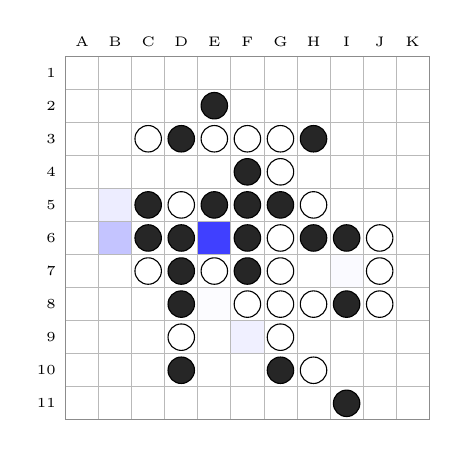
\begin{tikzpicture}[x=0.42cm, y=0.42cm]
\fill[blue!7] (1,-4) rectangle (2,-5);
\fill[blue!23] (1,-5) rectangle (2,-6);
\fill[blue!75] (4,-5) rectangle (5,-6);
\fill[blue!2] (8,-6) rectangle (9,-7);
\fill[blue!1] (4,-7) rectangle (5,-8);
\fill[blue!6] (5,-8) rectangle (6,-9);
\draw[gray!55, line width=.3pt, step=1] (0,0) grid (11,-11);
\draw[gray!90] (0,0) rectangle (11,-11);
\node[font=\tiny, anchor=south] at (0.5,0) {A};
\node[font=\tiny, anchor=south] at (1.5,0) {B};
\node[font=\tiny, anchor=south] at (2.5,0) {C};
\node[font=\tiny, anchor=south] at (3.5,0) {D};
\node[font=\tiny, anchor=south] at (4.5,0) {E};
\node[font=\tiny, anchor=south] at (5.5,0) {F};
\node[font=\tiny, anchor=south] at (6.5,0) {G};
\node[font=\tiny, anchor=south] at (7.5,0) {H};
\node[font=\tiny, anchor=south] at (8.5,0) {I};
\node[font=\tiny, anchor=south] at (9.5,0) {J};
\node[font=\tiny, anchor=south] at (10.5,0) {K};
\node[font=\tiny, anchor=east] at (0,-0.5) {1};
\node[font=\tiny, anchor=east] at (0,-1.5) {2};
\node[font=\tiny, anchor=east] at (0,-2.5) {3};
\node[font=\tiny, anchor=east] at (0,-3.5) {4};
\node[font=\tiny, anchor=east] at (0,-4.5) {5};
\node[font=\tiny, anchor=east] at (0,-5.5) {6};
\node[font=\tiny, anchor=east] at (0,-6.5) {7};
\node[font=\tiny, anchor=east] at (0,-7.5) {8};
\node[font=\tiny, anchor=east] at (0,-8.5) {9};
\node[font=\tiny, anchor=east] at (0,-9.5) {10};
\node[font=\tiny, anchor=east] at (0,-10.5) {11};
\draw[fill=black!85, line width=.4pt] (4.5,-1.5) circle (.40);
\draw[fill=white, line width=.4pt] (2.5,-2.5) circle (.40);
\draw[fill=black!85, line width=.4pt] (3.5,-2.5) circle (.40);
\draw[fill=white, line width=.4pt] (4.5,-2.5) circle (.40);
\draw[fill=white, line width=.4pt] (5.5,-2.5) circle (.40);
\draw[fill=white, line width=.4pt] (6.5,-2.5) circle (.40);
\draw[fill=black!85, line width=.4pt] (7.5,-2.5) circle (.40);
\draw[fill=black!85, line width=.4pt] (5.5,-3.5) circle (.40);
\draw[fill=white, line width=.4pt] (6.5,-3.5) circle (.40);
\draw[fill=black!85, line width=.4pt] (2.5,-4.5) circle (.40);
\draw[fill=white, line width=.4pt] (3.5,-4.5) circle (.40);
\draw[fill=black!85, line width=.4pt] (4.5,-4.5) circle (.40);
\draw[fill=black!85, line width=.4pt] (5.5,-4.5) circle (.40);
\draw[fill=black!85, line width=.4pt] (6.5,-4.5) circle (.40);
\draw[fill=white, line width=.4pt] (7.5,-4.5) circle (.40);
\draw[fill=black!85, line width=.4pt] (2.5,-5.5) circle (.40);
\draw[fill=black!85, line width=.4pt] (3.5,-5.5) circle (.40);
\draw[fill=black!85, line width=.4pt] (5.5,-5.5) circle (.40);
\draw[fill=white, line width=.4pt] (6.5,-5.5) circle (.40);
\draw[fill=black!85, line width=.4pt] (7.5,-5.5) circle (.40);
\draw[fill=black!85, line width=.4pt] (8.5,-5.5) circle (.40);
\draw[fill=white, line width=.4pt] (9.5,-5.5) circle (.40);
\draw[fill=white, line width=.4pt] (2.5,-6.5) circle (.40);
\draw[fill=black!85, line width=.4pt] (3.5,-6.5) circle (.40);
\draw[fill=white, line width=.4pt] (4.5,-6.5) circle (.40);
\draw[fill=black!85, line width=.4pt] (5.5,-6.5) circle (.40);
\draw[fill=white, line width=.4pt] (6.5,-6.5) circle (.40);
\draw[fill=white, line width=.4pt] (9.5,-6.5) circle (.40);
\draw[fill=black!85, line width=.4pt] (3.5,-7.5) circle (.40);
\draw[fill=white, line width=.4pt] (5.5,-7.5) circle (.40);
\draw[fill=white, line width=.4pt] (6.5,-7.5) circle (.40);
\draw[fill=white, line width=.4pt] (7.5,-7.5) circle (.40);
\draw[fill=black!85, line width=.4pt] (8.5,-7.5) circle (.40);
\draw[fill=white, line width=.4pt] (9.5,-7.5) circle (.40);
\draw[fill=white, line width=.4pt] (3.5,-8.5) circle (.40);
\draw[fill=white, line width=.4pt] (6.5,-8.5) circle (.40);
\draw[fill=black!85, line width=.4pt] (3.5,-9.5) circle (.40);
\draw[fill=black!85, line width=.4pt] (6.5,-9.5) circle (.40);
\draw[fill=white, line width=.4pt] (7.5,-9.5) circle (.40);
\draw[fill=black!85, line width=.4pt] (8.5,-10.5) circle (.40);
\end{tikzpicture}
    \caption{SL không aug: $v=0{,}60$; đáp án 86,8\%; cao nhất E6 (66,3\%)}
  \end{subfigure}\par\medskip
  \begin{subfigure}[t]{.48\linewidth}
    \centering
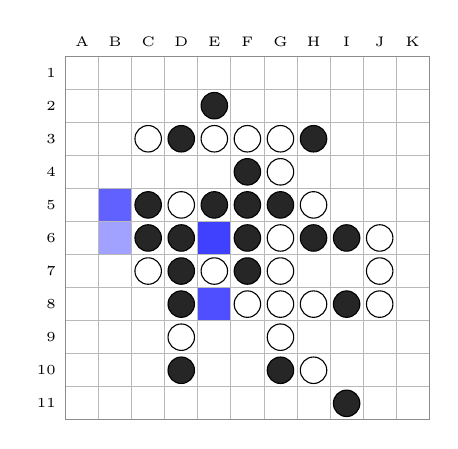
\begin{tikzpicture}[x=0.42cm, y=0.42cm]
\fill[blue!62] (1,-4) rectangle (2,-5);
\fill[blue!37] (1,-5) rectangle (2,-6);
\fill[blue!75] (4,-5) rectangle (5,-6);
\fill[blue!69] (4,-7) rectangle (5,-8);
\draw[gray!55, line width=.3pt, step=1] (0,0) grid (11,-11);
\draw[gray!90] (0,0) rectangle (11,-11);
\node[font=\tiny, anchor=south] at (0.5,0) {A};
\node[font=\tiny, anchor=south] at (1.5,0) {B};
\node[font=\tiny, anchor=south] at (2.5,0) {C};
\node[font=\tiny, anchor=south] at (3.5,0) {D};
\node[font=\tiny, anchor=south] at (4.5,0) {E};
\node[font=\tiny, anchor=south] at (5.5,0) {F};
\node[font=\tiny, anchor=south] at (6.5,0) {G};
\node[font=\tiny, anchor=south] at (7.5,0) {H};
\node[font=\tiny, anchor=south] at (8.5,0) {I};
\node[font=\tiny, anchor=south] at (9.5,0) {J};
\node[font=\tiny, anchor=south] at (10.5,0) {K};
\node[font=\tiny, anchor=east] at (0,-0.5) {1};
\node[font=\tiny, anchor=east] at (0,-1.5) {2};
\node[font=\tiny, anchor=east] at (0,-2.5) {3};
\node[font=\tiny, anchor=east] at (0,-3.5) {4};
\node[font=\tiny, anchor=east] at (0,-4.5) {5};
\node[font=\tiny, anchor=east] at (0,-5.5) {6};
\node[font=\tiny, anchor=east] at (0,-6.5) {7};
\node[font=\tiny, anchor=east] at (0,-7.5) {8};
\node[font=\tiny, anchor=east] at (0,-8.5) {9};
\node[font=\tiny, anchor=east] at (0,-9.5) {10};
\node[font=\tiny, anchor=east] at (0,-10.5) {11};
\draw[fill=black!85, line width=.4pt] (4.5,-1.5) circle (.40);
\draw[fill=white, line width=.4pt] (2.5,-2.5) circle (.40);
\draw[fill=black!85, line width=.4pt] (3.5,-2.5) circle (.40);
\draw[fill=white, line width=.4pt] (4.5,-2.5) circle (.40);
\draw[fill=white, line width=.4pt] (5.5,-2.5) circle (.40);
\draw[fill=white, line width=.4pt] (6.5,-2.5) circle (.40);
\draw[fill=black!85, line width=.4pt] (7.5,-2.5) circle (.40);
\draw[fill=black!85, line width=.4pt] (5.5,-3.5) circle (.40);
\draw[fill=white, line width=.4pt] (6.5,-3.5) circle (.40);
\draw[fill=black!85, line width=.4pt] (2.5,-4.5) circle (.40);
\draw[fill=white, line width=.4pt] (3.5,-4.5) circle (.40);
\draw[fill=black!85, line width=.4pt] (4.5,-4.5) circle (.40);
\draw[fill=black!85, line width=.4pt] (5.5,-4.5) circle (.40);
\draw[fill=black!85, line width=.4pt] (6.5,-4.5) circle (.40);
\draw[fill=white, line width=.4pt] (7.5,-4.5) circle (.40);
\draw[fill=black!85, line width=.4pt] (2.5,-5.5) circle (.40);
\draw[fill=black!85, line width=.4pt] (3.5,-5.5) circle (.40);
\draw[fill=black!85, line width=.4pt] (5.5,-5.5) circle (.40);
\draw[fill=white, line width=.4pt] (6.5,-5.5) circle (.40);
\draw[fill=black!85, line width=.4pt] (7.5,-5.5) circle (.40);
\draw[fill=black!85, line width=.4pt] (8.5,-5.5) circle (.40);
\draw[fill=white, line width=.4pt] (9.5,-5.5) circle (.40);
\draw[fill=white, line width=.4pt] (2.5,-6.5) circle (.40);
\draw[fill=black!85, line width=.4pt] (3.5,-6.5) circle (.40);
\draw[fill=white, line width=.4pt] (4.5,-6.5) circle (.40);
\draw[fill=black!85, line width=.4pt] (5.5,-6.5) circle (.40);
\draw[fill=white, line width=.4pt] (6.5,-6.5) circle (.40);
\draw[fill=white, line width=.4pt] (9.5,-6.5) circle (.40);
\draw[fill=black!85, line width=.4pt] (3.5,-7.5) circle (.40);
\draw[fill=white, line width=.4pt] (5.5,-7.5) circle (.40);
\draw[fill=white, line width=.4pt] (6.5,-7.5) circle (.40);
\draw[fill=white, line width=.4pt] (7.5,-7.5) circle (.40);
\draw[fill=black!85, line width=.4pt] (8.5,-7.5) circle (.40);
\draw[fill=white, line width=.4pt] (9.5,-7.5) circle (.40);
\draw[fill=white, line width=.4pt] (3.5,-8.5) circle (.40);
\draw[fill=white, line width=.4pt] (6.5,-8.5) circle (.40);
\draw[fill=black!85, line width=.4pt] (3.5,-9.5) circle (.40);
\draw[fill=black!85, line width=.4pt] (6.5,-9.5) circle (.40);
\draw[fill=white, line width=.4pt] (7.5,-9.5) circle (.40);
\draw[fill=black!85, line width=.4pt] (8.5,-10.5) circle (.40);
\end{tikzpicture}
    \caption{L6 (RL): $v=-0{,}30$; đáp án 73,9\%; cao nhất E6 (30,6\%)}
  \end{subfigure}\hfill
  \begin{subfigure}[t]{.48\linewidth}
    \centering
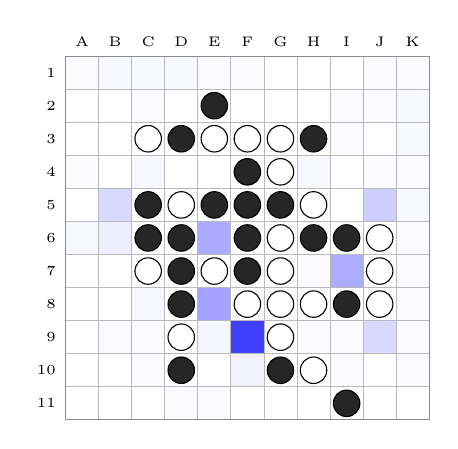
\begin{tikzpicture}[x=0.42cm, y=0.42cm]
\fill[blue!2] (0,0) rectangle (1,-1);
\fill[blue!3] (1,0) rectangle (2,-1);
\fill[blue!3] (2,0) rectangle (3,-1);
\fill[blue!3] (3,0) rectangle (4,-1);
\fill[blue!2] (4,0) rectangle (5,-1);
\fill[blue!2] (5,0) rectangle (6,-1);
\fill[blue!2] (9,0) rectangle (10,-1);
\fill[blue!2] (10,0) rectangle (11,-1);
\fill[blue!2] (2,-1) rectangle (3,-2);
\fill[blue!2] (8,-1) rectangle (9,-2);
\fill[blue!2] (9,-1) rectangle (10,-2);
\fill[blue!3] (10,-1) rectangle (11,-2);
\fill[blue!2] (8,-2) rectangle (9,-3);
\fill[blue!3] (10,-2) rectangle (11,-3);
\fill[blue!2] (0,-3) rectangle (1,-4);
\fill[blue!3] (2,-3) rectangle (3,-4);
\fill[blue!3] (7,-3) rectangle (8,-4);
\fill[blue!2] (9,-3) rectangle (10,-4);
\fill[blue!2] (10,-3) rectangle (11,-4);
\fill[blue!15] (1,-4) rectangle (2,-5);
\fill[blue!19] (9,-4) rectangle (10,-5);
\fill[blue!3] (10,-4) rectangle (11,-5);
\fill[blue!3] (0,-5) rectangle (1,-6);
\fill[blue!7] (1,-5) rectangle (2,-6);
\fill[blue!33] (4,-5) rectangle (5,-6);
\fill[blue!2] (10,-5) rectangle (11,-6);
\fill[blue!2] (7,-6) rectangle (8,-7);
\fill[blue!32] (8,-6) rectangle (9,-7);
\fill[blue!2] (10,-6) rectangle (11,-7);
\fill[blue!3] (2,-7) rectangle (3,-8);
\fill[blue!36] (4,-7) rectangle (5,-8);
\fill[blue!2] (10,-7) rectangle (11,-8);
\fill[blue!2] (1,-8) rectangle (2,-9);
\fill[blue!2] (2,-8) rectangle (3,-9);
\fill[blue!4] (4,-8) rectangle (5,-9);
\fill[blue!75] (5,-8) rectangle (6,-9);
\fill[blue!2] (7,-8) rectangle (8,-9);
\fill[blue!2] (8,-8) rectangle (9,-9);
\fill[blue!15] (9,-8) rectangle (10,-9);
\fill[blue!2] (10,-8) rectangle (11,-9);
\fill[blue!2] (2,-9) rectangle (3,-10);
\fill[blue!5] (5,-9) rectangle (6,-10);
\fill[blue!2] (8,-9) rectangle (9,-10);
\fill[blue!2] (10,-9) rectangle (11,-10);
\fill[blue!2] (3,-10) rectangle (4,-11);
\fill[blue!2] (4,-10) rectangle (5,-11);
\draw[gray!55, line width=.3pt, step=1] (0,0) grid (11,-11);
\draw[gray!90] (0,0) rectangle (11,-11);
\node[font=\tiny, anchor=south] at (0.5,0) {A};
\node[font=\tiny, anchor=south] at (1.5,0) {B};
\node[font=\tiny, anchor=south] at (2.5,0) {C};
\node[font=\tiny, anchor=south] at (3.5,0) {D};
\node[font=\tiny, anchor=south] at (4.5,0) {E};
\node[font=\tiny, anchor=south] at (5.5,0) {F};
\node[font=\tiny, anchor=south] at (6.5,0) {G};
\node[font=\tiny, anchor=south] at (7.5,0) {H};
\node[font=\tiny, anchor=south] at (8.5,0) {I};
\node[font=\tiny, anchor=south] at (9.5,0) {J};
\node[font=\tiny, anchor=south] at (10.5,0) {K};
\node[font=\tiny, anchor=east] at (0,-0.5) {1};
\node[font=\tiny, anchor=east] at (0,-1.5) {2};
\node[font=\tiny, anchor=east] at (0,-2.5) {3};
\node[font=\tiny, anchor=east] at (0,-3.5) {4};
\node[font=\tiny, anchor=east] at (0,-4.5) {5};
\node[font=\tiny, anchor=east] at (0,-5.5) {6};
\node[font=\tiny, anchor=east] at (0,-6.5) {7};
\node[font=\tiny, anchor=east] at (0,-7.5) {8};
\node[font=\tiny, anchor=east] at (0,-8.5) {9};
\node[font=\tiny, anchor=east] at (0,-9.5) {10};
\node[font=\tiny, anchor=east] at (0,-10.5) {11};
\draw[fill=black!85, line width=.4pt] (4.5,-1.5) circle (.40);
\draw[fill=white, line width=.4pt] (2.5,-2.5) circle (.40);
\draw[fill=black!85, line width=.4pt] (3.5,-2.5) circle (.40);
\draw[fill=white, line width=.4pt] (4.5,-2.5) circle (.40);
\draw[fill=white, line width=.4pt] (5.5,-2.5) circle (.40);
\draw[fill=white, line width=.4pt] (6.5,-2.5) circle (.40);
\draw[fill=black!85, line width=.4pt] (7.5,-2.5) circle (.40);
\draw[fill=black!85, line width=.4pt] (5.5,-3.5) circle (.40);
\draw[fill=white, line width=.4pt] (6.5,-3.5) circle (.40);
\draw[fill=black!85, line width=.4pt] (2.5,-4.5) circle (.40);
\draw[fill=white, line width=.4pt] (3.5,-4.5) circle (.40);
\draw[fill=black!85, line width=.4pt] (4.5,-4.5) circle (.40);
\draw[fill=black!85, line width=.4pt] (5.5,-4.5) circle (.40);
\draw[fill=black!85, line width=.4pt] (6.5,-4.5) circle (.40);
\draw[fill=white, line width=.4pt] (7.5,-4.5) circle (.40);
\draw[fill=black!85, line width=.4pt] (2.5,-5.5) circle (.40);
\draw[fill=black!85, line width=.4pt] (3.5,-5.5) circle (.40);
\draw[fill=black!85, line width=.4pt] (5.5,-5.5) circle (.40);
\draw[fill=white, line width=.4pt] (6.5,-5.5) circle (.40);
\draw[fill=black!85, line width=.4pt] (7.5,-5.5) circle (.40);
\draw[fill=black!85, line width=.4pt] (8.5,-5.5) circle (.40);
\draw[fill=white, line width=.4pt] (9.5,-5.5) circle (.40);
\draw[fill=white, line width=.4pt] (2.5,-6.5) circle (.40);
\draw[fill=black!85, line width=.4pt] (3.5,-6.5) circle (.40);
\draw[fill=white, line width=.4pt] (4.5,-6.5) circle (.40);
\draw[fill=black!85, line width=.4pt] (5.5,-6.5) circle (.40);
\draw[fill=white, line width=.4pt] (6.5,-6.5) circle (.40);
\draw[fill=white, line width=.4pt] (9.5,-6.5) circle (.40);
\draw[fill=black!85, line width=.4pt] (3.5,-7.5) circle (.40);
\draw[fill=white, line width=.4pt] (5.5,-7.5) circle (.40);
\draw[fill=white, line width=.4pt] (6.5,-7.5) circle (.40);
\draw[fill=white, line width=.4pt] (7.5,-7.5) circle (.40);
\draw[fill=black!85, line width=.4pt] (8.5,-7.5) circle (.40);
\draw[fill=white, line width=.4pt] (9.5,-7.5) circle (.40);
\draw[fill=white, line width=.4pt] (3.5,-8.5) circle (.40);
\draw[fill=white, line width=.4pt] (6.5,-8.5) circle (.40);
\draw[fill=black!85, line width=.4pt] (3.5,-9.5) circle (.40);
\draw[fill=black!85, line width=.4pt] (6.5,-9.5) circle (.40);
\draw[fill=white, line width=.4pt] (7.5,-9.5) circle (.40);
\draw[fill=black!85, line width=.4pt] (8.5,-10.5) circle (.40);
\end{tikzpicture}
    \caption{L8 (AZ): $v=-0{,}73$; đáp án 20,0\%; cao nhất F9 (19,9\%)}
  \end{subfigure}\par\medskip
  \caption{Policy của bốn mạng tại thế C4-001 (X đi). Ô càng đậm xác suất càng cao (chuẩn hoá theo ô lớn nhất của từng mạng). Đáp án: B6, E6, E8.}
  \label{fig:cs-policy-c4}
\end{figure}

\begin{figure}[H]
  \centering
  \begin{subfigure}[t]{.48\linewidth}
    \centering
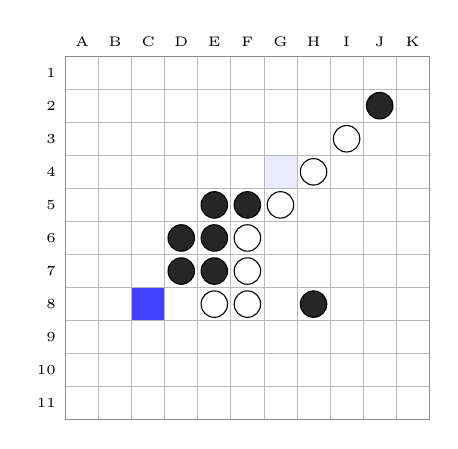
\begin{tikzpicture}[x=0.42cm, y=0.42cm]
\fill[blue!8] (6,-3) rectangle (7,-4);
\fill[blue!75] (2,-7) rectangle (3,-8);
\draw[gray!55, line width=.3pt, step=1] (0,0) grid (11,-11);
\draw[gray!90] (0,0) rectangle (11,-11);
\node[font=\tiny, anchor=south] at (0.5,0) {A};
\node[font=\tiny, anchor=south] at (1.5,0) {B};
\node[font=\tiny, anchor=south] at (2.5,0) {C};
\node[font=\tiny, anchor=south] at (3.5,0) {D};
\node[font=\tiny, anchor=south] at (4.5,0) {E};
\node[font=\tiny, anchor=south] at (5.5,0) {F};
\node[font=\tiny, anchor=south] at (6.5,0) {G};
\node[font=\tiny, anchor=south] at (7.5,0) {H};
\node[font=\tiny, anchor=south] at (8.5,0) {I};
\node[font=\tiny, anchor=south] at (9.5,0) {J};
\node[font=\tiny, anchor=south] at (10.5,0) {K};
\node[font=\tiny, anchor=east] at (0,-0.5) {1};
\node[font=\tiny, anchor=east] at (0,-1.5) {2};
\node[font=\tiny, anchor=east] at (0,-2.5) {3};
\node[font=\tiny, anchor=east] at (0,-3.5) {4};
\node[font=\tiny, anchor=east] at (0,-4.5) {5};
\node[font=\tiny, anchor=east] at (0,-5.5) {6};
\node[font=\tiny, anchor=east] at (0,-6.5) {7};
\node[font=\tiny, anchor=east] at (0,-7.5) {8};
\node[font=\tiny, anchor=east] at (0,-8.5) {9};
\node[font=\tiny, anchor=east] at (0,-9.5) {10};
\node[font=\tiny, anchor=east] at (0,-10.5) {11};
\draw[fill=black!85, line width=.4pt] (9.5,-1.5) circle (.40);
\draw[fill=white, line width=.4pt] (8.5,-2.5) circle (.40);
\draw[fill=white, line width=.4pt] (7.5,-3.5) circle (.40);
\draw[fill=black!85, line width=.4pt] (4.5,-4.5) circle (.40);
\draw[fill=black!85, line width=.4pt] (5.5,-4.5) circle (.40);
\draw[fill=white, line width=.4pt] (6.5,-4.5) circle (.40);
\draw[fill=black!85, line width=.4pt] (3.5,-5.5) circle (.40);
\draw[fill=black!85, line width=.4pt] (4.5,-5.5) circle (.40);
\draw[fill=white, line width=.4pt] (5.5,-5.5) circle (.40);
\draw[fill=black!85, line width=.4pt] (3.5,-6.5) circle (.40);
\draw[fill=black!85, line width=.4pt] (4.5,-6.5) circle (.40);
\draw[fill=white, line width=.4pt] (5.5,-6.5) circle (.40);
\draw[fill=white, line width=.4pt] (4.5,-7.5) circle (.40);
\draw[fill=white, line width=.4pt] (5.5,-7.5) circle (.40);
\draw[fill=black!85, line width=.4pt] (7.5,-7.5) circle (.40);
\end{tikzpicture}
    \caption{SL v3: $v=0{,}18$; đáp án 99,9\%; cao nhất C8 (90,4\%)}
  \end{subfigure}\hfill
  \begin{subfigure}[t]{.48\linewidth}
    \centering
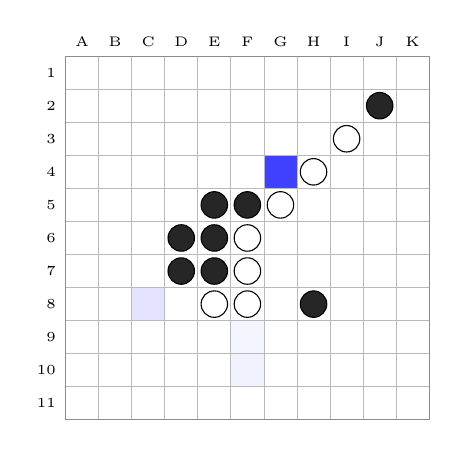
\begin{tikzpicture}[x=0.42cm, y=0.42cm]
\fill[blue!75] (6,-3) rectangle (7,-4);
\fill[blue!11] (2,-7) rectangle (3,-8);
\fill[blue!4] (5,-8) rectangle (6,-9);
\fill[blue!5] (5,-9) rectangle (6,-10);
\draw[gray!55, line width=.3pt, step=1] (0,0) grid (11,-11);
\draw[gray!90] (0,0) rectangle (11,-11);
\node[font=\tiny, anchor=south] at (0.5,0) {A};
\node[font=\tiny, anchor=south] at (1.5,0) {B};
\node[font=\tiny, anchor=south] at (2.5,0) {C};
\node[font=\tiny, anchor=south] at (3.5,0) {D};
\node[font=\tiny, anchor=south] at (4.5,0) {E};
\node[font=\tiny, anchor=south] at (5.5,0) {F};
\node[font=\tiny, anchor=south] at (6.5,0) {G};
\node[font=\tiny, anchor=south] at (7.5,0) {H};
\node[font=\tiny, anchor=south] at (8.5,0) {I};
\node[font=\tiny, anchor=south] at (9.5,0) {J};
\node[font=\tiny, anchor=south] at (10.5,0) {K};
\node[font=\tiny, anchor=east] at (0,-0.5) {1};
\node[font=\tiny, anchor=east] at (0,-1.5) {2};
\node[font=\tiny, anchor=east] at (0,-2.5) {3};
\node[font=\tiny, anchor=east] at (0,-3.5) {4};
\node[font=\tiny, anchor=east] at (0,-4.5) {5};
\node[font=\tiny, anchor=east] at (0,-5.5) {6};
\node[font=\tiny, anchor=east] at (0,-6.5) {7};
\node[font=\tiny, anchor=east] at (0,-7.5) {8};
\node[font=\tiny, anchor=east] at (0,-8.5) {9};
\node[font=\tiny, anchor=east] at (0,-9.5) {10};
\node[font=\tiny, anchor=east] at (0,-10.5) {11};
\draw[fill=black!85, line width=.4pt] (9.5,-1.5) circle (.40);
\draw[fill=white, line width=.4pt] (8.5,-2.5) circle (.40);
\draw[fill=white, line width=.4pt] (7.5,-3.5) circle (.40);
\draw[fill=black!85, line width=.4pt] (4.5,-4.5) circle (.40);
\draw[fill=black!85, line width=.4pt] (5.5,-4.5) circle (.40);
\draw[fill=white, line width=.4pt] (6.5,-4.5) circle (.40);
\draw[fill=black!85, line width=.4pt] (3.5,-5.5) circle (.40);
\draw[fill=black!85, line width=.4pt] (4.5,-5.5) circle (.40);
\draw[fill=white, line width=.4pt] (5.5,-5.5) circle (.40);
\draw[fill=black!85, line width=.4pt] (3.5,-6.5) circle (.40);
\draw[fill=black!85, line width=.4pt] (4.5,-6.5) circle (.40);
\draw[fill=white, line width=.4pt] (5.5,-6.5) circle (.40);
\draw[fill=white, line width=.4pt] (4.5,-7.5) circle (.40);
\draw[fill=white, line width=.4pt] (5.5,-7.5) circle (.40);
\draw[fill=black!85, line width=.4pt] (7.5,-7.5) circle (.40);
\end{tikzpicture}
    \caption{SL không aug: $v=-0{,}42$; đáp án 98,5\%; cao nhất G4 (78,0\%)}
  \end{subfigure}\par\medskip
  \begin{subfigure}[t]{.48\linewidth}
    \centering
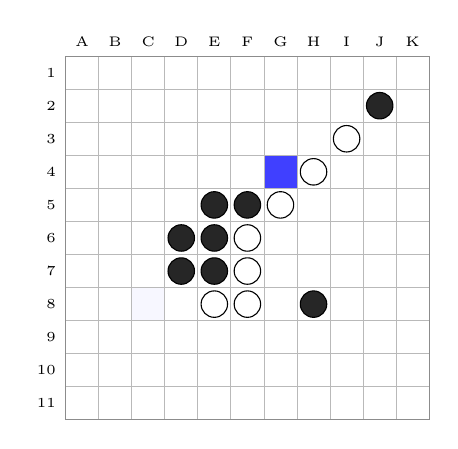
\begin{tikzpicture}[x=0.42cm, y=0.42cm]
\fill[blue!75] (6,-3) rectangle (7,-4);
\fill[blue!3] (2,-7) rectangle (3,-8);
\draw[gray!55, line width=.3pt, step=1] (0,0) grid (11,-11);
\draw[gray!90] (0,0) rectangle (11,-11);
\node[font=\tiny, anchor=south] at (0.5,0) {A};
\node[font=\tiny, anchor=south] at (1.5,0) {B};
\node[font=\tiny, anchor=south] at (2.5,0) {C};
\node[font=\tiny, anchor=south] at (3.5,0) {D};
\node[font=\tiny, anchor=south] at (4.5,0) {E};
\node[font=\tiny, anchor=south] at (5.5,0) {F};
\node[font=\tiny, anchor=south] at (6.5,0) {G};
\node[font=\tiny, anchor=south] at (7.5,0) {H};
\node[font=\tiny, anchor=south] at (8.5,0) {I};
\node[font=\tiny, anchor=south] at (9.5,0) {J};
\node[font=\tiny, anchor=south] at (10.5,0) {K};
\node[font=\tiny, anchor=east] at (0,-0.5) {1};
\node[font=\tiny, anchor=east] at (0,-1.5) {2};
\node[font=\tiny, anchor=east] at (0,-2.5) {3};
\node[font=\tiny, anchor=east] at (0,-3.5) {4};
\node[font=\tiny, anchor=east] at (0,-4.5) {5};
\node[font=\tiny, anchor=east] at (0,-5.5) {6};
\node[font=\tiny, anchor=east] at (0,-6.5) {7};
\node[font=\tiny, anchor=east] at (0,-7.5) {8};
\node[font=\tiny, anchor=east] at (0,-8.5) {9};
\node[font=\tiny, anchor=east] at (0,-9.5) {10};
\node[font=\tiny, anchor=east] at (0,-10.5) {11};
\draw[fill=black!85, line width=.4pt] (9.5,-1.5) circle (.40);
\draw[fill=white, line width=.4pt] (8.5,-2.5) circle (.40);
\draw[fill=white, line width=.4pt] (7.5,-3.5) circle (.40);
\draw[fill=black!85, line width=.4pt] (4.5,-4.5) circle (.40);
\draw[fill=black!85, line width=.4pt] (5.5,-4.5) circle (.40);
\draw[fill=white, line width=.4pt] (6.5,-4.5) circle (.40);
\draw[fill=black!85, line width=.4pt] (3.5,-5.5) circle (.40);
\draw[fill=black!85, line width=.4pt] (4.5,-5.5) circle (.40);
\draw[fill=white, line width=.4pt] (5.5,-5.5) circle (.40);
\draw[fill=black!85, line width=.4pt] (3.5,-6.5) circle (.40);
\draw[fill=black!85, line width=.4pt] (4.5,-6.5) circle (.40);
\draw[fill=white, line width=.4pt] (5.5,-6.5) circle (.40);
\draw[fill=white, line width=.4pt] (4.5,-7.5) circle (.40);
\draw[fill=white, line width=.4pt] (5.5,-7.5) circle (.40);
\draw[fill=black!85, line width=.4pt] (7.5,-7.5) circle (.40);
\end{tikzpicture}
    \caption{L6 (RL): $v=0{,}19$; đáp án 100,0\%; cao nhất G4 (95,6\%)}
  \end{subfigure}\hfill
  \begin{subfigure}[t]{.48\linewidth}
    \centering
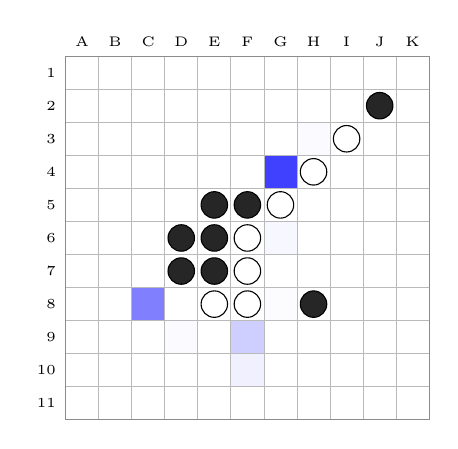
\begin{tikzpicture}[x=0.42cm, y=0.42cm]
\fill[blue!2] (7,-2) rectangle (8,-3);
\fill[blue!75] (6,-3) rectangle (7,-4);
\fill[blue!3] (6,-5) rectangle (7,-6);
\fill[blue!50] (2,-7) rectangle (3,-8);
\fill[blue!1] (6,-7) rectangle (7,-8);
\fill[blue!2] (3,-8) rectangle (4,-9);
\fill[blue!19] (5,-8) rectangle (6,-9);
\fill[blue!6] (5,-9) rectangle (6,-10);
\draw[gray!55, line width=.3pt, step=1] (0,0) grid (11,-11);
\draw[gray!90] (0,0) rectangle (11,-11);
\node[font=\tiny, anchor=south] at (0.5,0) {A};
\node[font=\tiny, anchor=south] at (1.5,0) {B};
\node[font=\tiny, anchor=south] at (2.5,0) {C};
\node[font=\tiny, anchor=south] at (3.5,0) {D};
\node[font=\tiny, anchor=south] at (4.5,0) {E};
\node[font=\tiny, anchor=south] at (5.5,0) {F};
\node[font=\tiny, anchor=south] at (6.5,0) {G};
\node[font=\tiny, anchor=south] at (7.5,0) {H};
\node[font=\tiny, anchor=south] at (8.5,0) {I};
\node[font=\tiny, anchor=south] at (9.5,0) {J};
\node[font=\tiny, anchor=south] at (10.5,0) {K};
\node[font=\tiny, anchor=east] at (0,-0.5) {1};
\node[font=\tiny, anchor=east] at (0,-1.5) {2};
\node[font=\tiny, anchor=east] at (0,-2.5) {3};
\node[font=\tiny, anchor=east] at (0,-3.5) {4};
\node[font=\tiny, anchor=east] at (0,-4.5) {5};
\node[font=\tiny, anchor=east] at (0,-5.5) {6};
\node[font=\tiny, anchor=east] at (0,-6.5) {7};
\node[font=\tiny, anchor=east] at (0,-7.5) {8};
\node[font=\tiny, anchor=east] at (0,-8.5) {9};
\node[font=\tiny, anchor=east] at (0,-9.5) {10};
\node[font=\tiny, anchor=east] at (0,-10.5) {11};
\draw[fill=black!85, line width=.4pt] (9.5,-1.5) circle (.40);
\draw[fill=white, line width=.4pt] (8.5,-2.5) circle (.40);
\draw[fill=white, line width=.4pt] (7.5,-3.5) circle (.40);
\draw[fill=black!85, line width=.4pt] (4.5,-4.5) circle (.40);
\draw[fill=black!85, line width=.4pt] (5.5,-4.5) circle (.40);
\draw[fill=white, line width=.4pt] (6.5,-4.5) circle (.40);
\draw[fill=black!85, line width=.4pt] (3.5,-5.5) circle (.40);
\draw[fill=black!85, line width=.4pt] (4.5,-5.5) circle (.40);
\draw[fill=white, line width=.4pt] (5.5,-5.5) circle (.40);
\draw[fill=black!85, line width=.4pt] (3.5,-6.5) circle (.40);
\draw[fill=black!85, line width=.4pt] (4.5,-6.5) circle (.40);
\draw[fill=white, line width=.4pt] (5.5,-6.5) circle (.40);
\draw[fill=white, line width=.4pt] (4.5,-7.5) circle (.40);
\draw[fill=white, line width=.4pt] (5.5,-7.5) circle (.40);
\draw[fill=black!85, line width=.4pt] (7.5,-7.5) circle (.40);
\end{tikzpicture}
    \caption{L8 (AZ): $v=-0{,}78$; đáp án 64,4\%; cao nhất G4 (32,3\%)}
  \end{subfigure}\par\medskip
  \caption{Policy của bốn mạng tại thế C5-001 (O đi). Ô càng đậm xác suất càng cao (chuẩn hoá theo ô lớn nhất của từng mạng). Đáp án: G4, C8, F9, F10.}
  \label{fig:cs-policy-c5}
\end{figure}


\subsection{Quỹ đạo giá trị trong ván L7 gặp L8}
\begin{figure}[H]
  \centering
  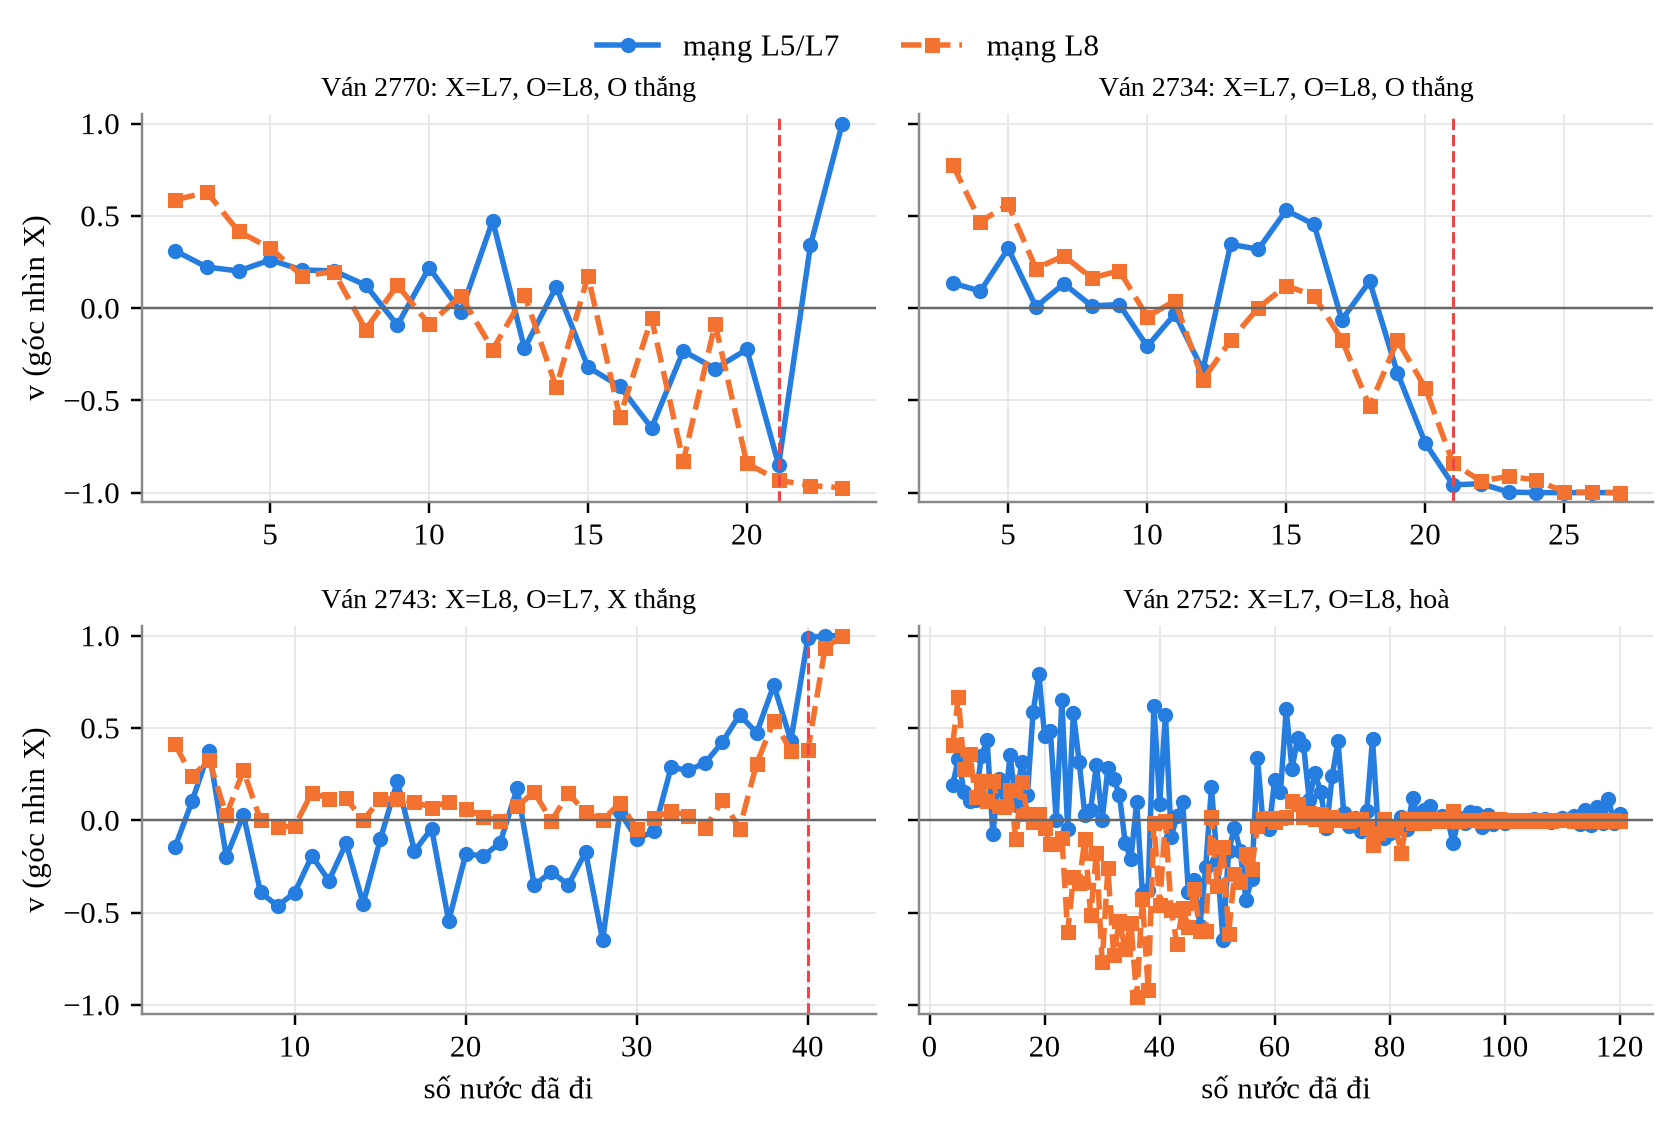
\includegraphics[width=\linewidth]{chuyen-sau/hinh/mang-quy-dao.png}
  \caption{Giá trị (đổi về góc nhìn X) của hai mạng theo từng nước trong bốn ván L7 gặp L8, chọn theo phân vị độ dài
  25\%, 50\%, 75\% và 95\%. Đường đỏ đứt: thế đầu tiên có bên đi có VCF.}
  \label{fig:cs-mang-quy-dao}
\end{figure}
Bốn ván được chọn theo độ dài, không theo kết quả. Mạng L5 dao động mạnh giữa hai nước liên tiếp (đổi góc nhìn làm lộ
ra phần đánh giá phụ thuộc bên đi), còn mạng L8 mượt hơn ở đầu ván. Ở các ván có thắng thua, cả hai mạng thường chỉ
nghiêng hẳn về bên thắng gần thời điểm VCF xuất hiện. Bốn ván không đủ để so định lượng hai value head; chúng minh hoạ
vì sao một giá trị lá chính xác ở trung cuộc khó hơn nhiều ở thế đã có đe doạ.
